% ============================================================================
%  A0 portrait scientific poster  (compile with pdflatex)
%  Carbon-Intelligent Workload Scheduling for AI Data Centers
%  Dense 3-column grid; navy/blue theme harmonised with the thesis (ieblue)
%  and the SciencePlots figure palette (#0C5DA5 blue, #00B945 green).
% ============================================================================
\documentclass[final]{beamer}
\usepackage[size=a0,orientation=portrait,scale=1.0]{beamerposter}
\usetheme{default}
\usefonttheme{serif}                 % use the document serif font everywhere
\usepackage[T1]{fontenc}
\let\Bbbk\relax
\usepackage{newtxtext,newtxmath}     % Times serif, unified with thesis + figures
\usepackage{graphicx}
\usepackage{amsmath}
\usepackage{booktabs}
\usepackage{array}
\usepackage{tabularx}
\usepackage{colortbl}
\usepackage{pifont}
\graphicspath{{figures/results/}{figures/eda/}}

% ── Low-saturation sage-green theme ─────────────────────────────────────────
\definecolor{pdark}{RGB}{52,80,63}     % deep sage green — section headers / title
\definecolor{pmid}{RGB}{96,130,106}    % muted green — accent
\definecolor{pgreen}{RGB}{42,120,72}   % green — positive accent
\definecolor{pred}{RGB}{190,78,62}     % muted terracotta — negative accent
\definecolor{ptint}{RGB}{240,244,240}  % very light green — card body
\definecolor{pcard}{RGB}{224,233,226}  % light green — metric cards
\definecolor{phl}{RGB}{210,224,213}    % highlight band

\newcommand{\yes}{\textcolor{pgreen}{\ding{51}}}
\newcommand{\no}{\textcolor{pred}{\ding{55}}}

\setbeamercolor{block title}{bg=pdark,fg=white}
\setbeamercolor{block body}{bg=ptint,fg=black}
\setbeamercolor{metric}{bg=pcard,fg=pdark}
\setbeamercolor{hl}{bg=phl,fg=pdark}

\setbeamertemplate{block begin}{
  \vskip0.1ex
  \begin{beamercolorbox}[ht=2.5ex,dp=0.85ex,leftskip=0.5cm,rounded=true]{block title}
    \usebeamerfont{block title}\bfseries\insertblocktitle
  \end{beamercolorbox}
  \vskip-0.15ex
  \begin{beamercolorbox}[leftskip=0.55cm,rightskip=0.55cm,vmode,rounded=true]{block body}
  \vskip0.7ex
}
\setbeamertemplate{block end}{\vskip0.8ex\end{beamercolorbox}\vskip1.1ex}
\setbeamertemplate{navigation symbols}{}
\setbeamerfont{block title}{series=\bfseries,size=\large}
\setbeamerfont{block body}{size=\footnotesize}   % uniform body text size everywhere

\newlength{\colw}\setlength{\colw}{0.312\paperwidth}
\newlength{\colht}\setlength{\colht}{0.845\paperheight}  % fixed column height; \vfill fills it
\newcommand{\sn}[1]{{\color{white}\fontsize{26}{26}\selectfont\bfseries #1}\,\ }
\newcommand{\metric}[2]{%
\begin{minipage}{0.235\paperwidth}\centering
\begin{beamercolorbox}[wd=\linewidth,sep=0.3cm,center,rounded=true]{metric}
{\fontsize{42}{48}\selectfont\bfseries #1}\\[0.8mm]{\small #2}
\end{beamercolorbox}\end{minipage}}
\newcommand{\finding}[2]{%
\begin{minipage}{0.315\paperwidth}\centering
\begin{beamercolorbox}[wd=\linewidth,sep=0.3cm,rounded=true]{hl}
{\fontsize{22}{26}\selectfont\bfseries #1}\\[1mm]{\small #2}
\end{beamercolorbox}\end{minipage}}
\newenvironment{callout}{\begin{beamercolorbox}[sep=0.4cm,rounded=true]{hl}}{\end{beamercolorbox}\vskip0.2ex}

% compact caption command for figures inside blocks
\newcommand{\fcap}[1]{\par\vskip0.15ex{\footnotesize #1}}

\begin{document}
\begin{frame}[t]{}

% ── Hero header ─────────────────────────────────────────────────────────────
\begin{beamercolorbox}[wd=\paperwidth,sep=0.8cm]{block title}
\centering
{\fontsize{60}{68}\selectfont\bfseries Carbon-Intelligent Workload Scheduling for AI Data Centers}\\[3.5mm]
{\fontsize{30}{36}\selectfont A Deterministic Optimization Approach to Joint Temporal and Spatial Scheduling}\\[4.5mm]
{\large Yaxin Wu \quad\textbullet\quad Supervisor: Prof.\ Bissan Ghaddar \quad\textbullet\quad MBDS, IE University}
\end{beamercolorbox}
\vspace{0.28cm}

% ── Core findings band (conclusions on top) ─────────────────────────────────
\centering
\finding{Routing $>$ Timing}{Carbon savings come from \emph{where} load runs, not \emph{when}}\hfill
\finding{Geography is the lever}{Geographic flexibility dominates every other parameter by $\sim\!10\times$}\hfill
\finding{Large, robust savings}{Up to \textbf{78\%} carbon cut; \textbf{31\%} under full operational limits}
\vspace{0.18cm}

% ── Metric strip ────────────────────────────────────────────────────────────
\metric{78\%}{max carbon cut\\(vs.\ no optimization)}\hfill
\metric{31\%}{under full\\operational constraints}\hfill
\metric{$\times$10}{geographic flexibility\\over any parameter}\hfill
\metric{5\,/\,2\,yr}{grids backtested\\over 2024--2025}
\vspace{0.16cm}

% ===================== THREE COLUMNS =====================
\begin{columns}[t]

% =========================== COLUMN 1 ===========================
\begin{column}{\colw}
\begin{minipage}[t][\colht]{\linewidth}

\begin{block}{\sn{1} Motivation \& Research Question}
AI electricity demand is growing faster than grids can decarbonize, making the \textbf{operational carbon} of computing a first-order concern. Grid \textbf{carbon intensity (CI)} varies across \textbf{hours} and \textbf{regions}, so flexible load can move toward cleaner electricity. Existing schedulers are either \textbf{heuristic} (no optimality guarantee) or optimize the temporal and spatial dimensions \textbf{separately}.
\vskip0.45ex
\begin{callout}
\textit{How can a deterministic model minimize carbon through \textbf{joint} temporal and spatial scheduling across regions, subject to realistic operational constraints?}
\end{callout}
\end{block}
\vfill
\begin{block}{\sn{2} The Optimization Model}
A linear program chooses the flexible load $x_{r,t}$ in each region $r$ and hour $t$, driven by carbon intensity and the carbon-free energy fraction, to minimize operational carbon subject to seven operational constraints:
\vskip0.5ex
\centering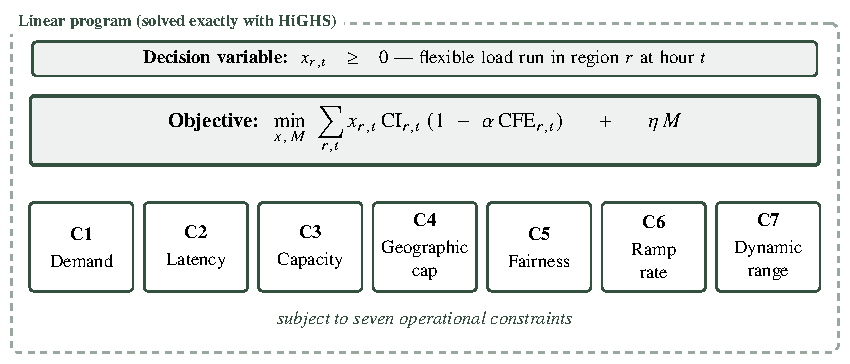
\includegraphics[width=\linewidth]{model_lp}
\end{block}
\vfill
\begin{block}{\sn{3} Carbon Data: Five Grid Regions}
Hourly CI and CFE from \textbf{ElectricityMaps}, \textbf{2024--2025} ($17{,}544$\,h $\times$ 5 grids).
\vskip0.3ex
\centering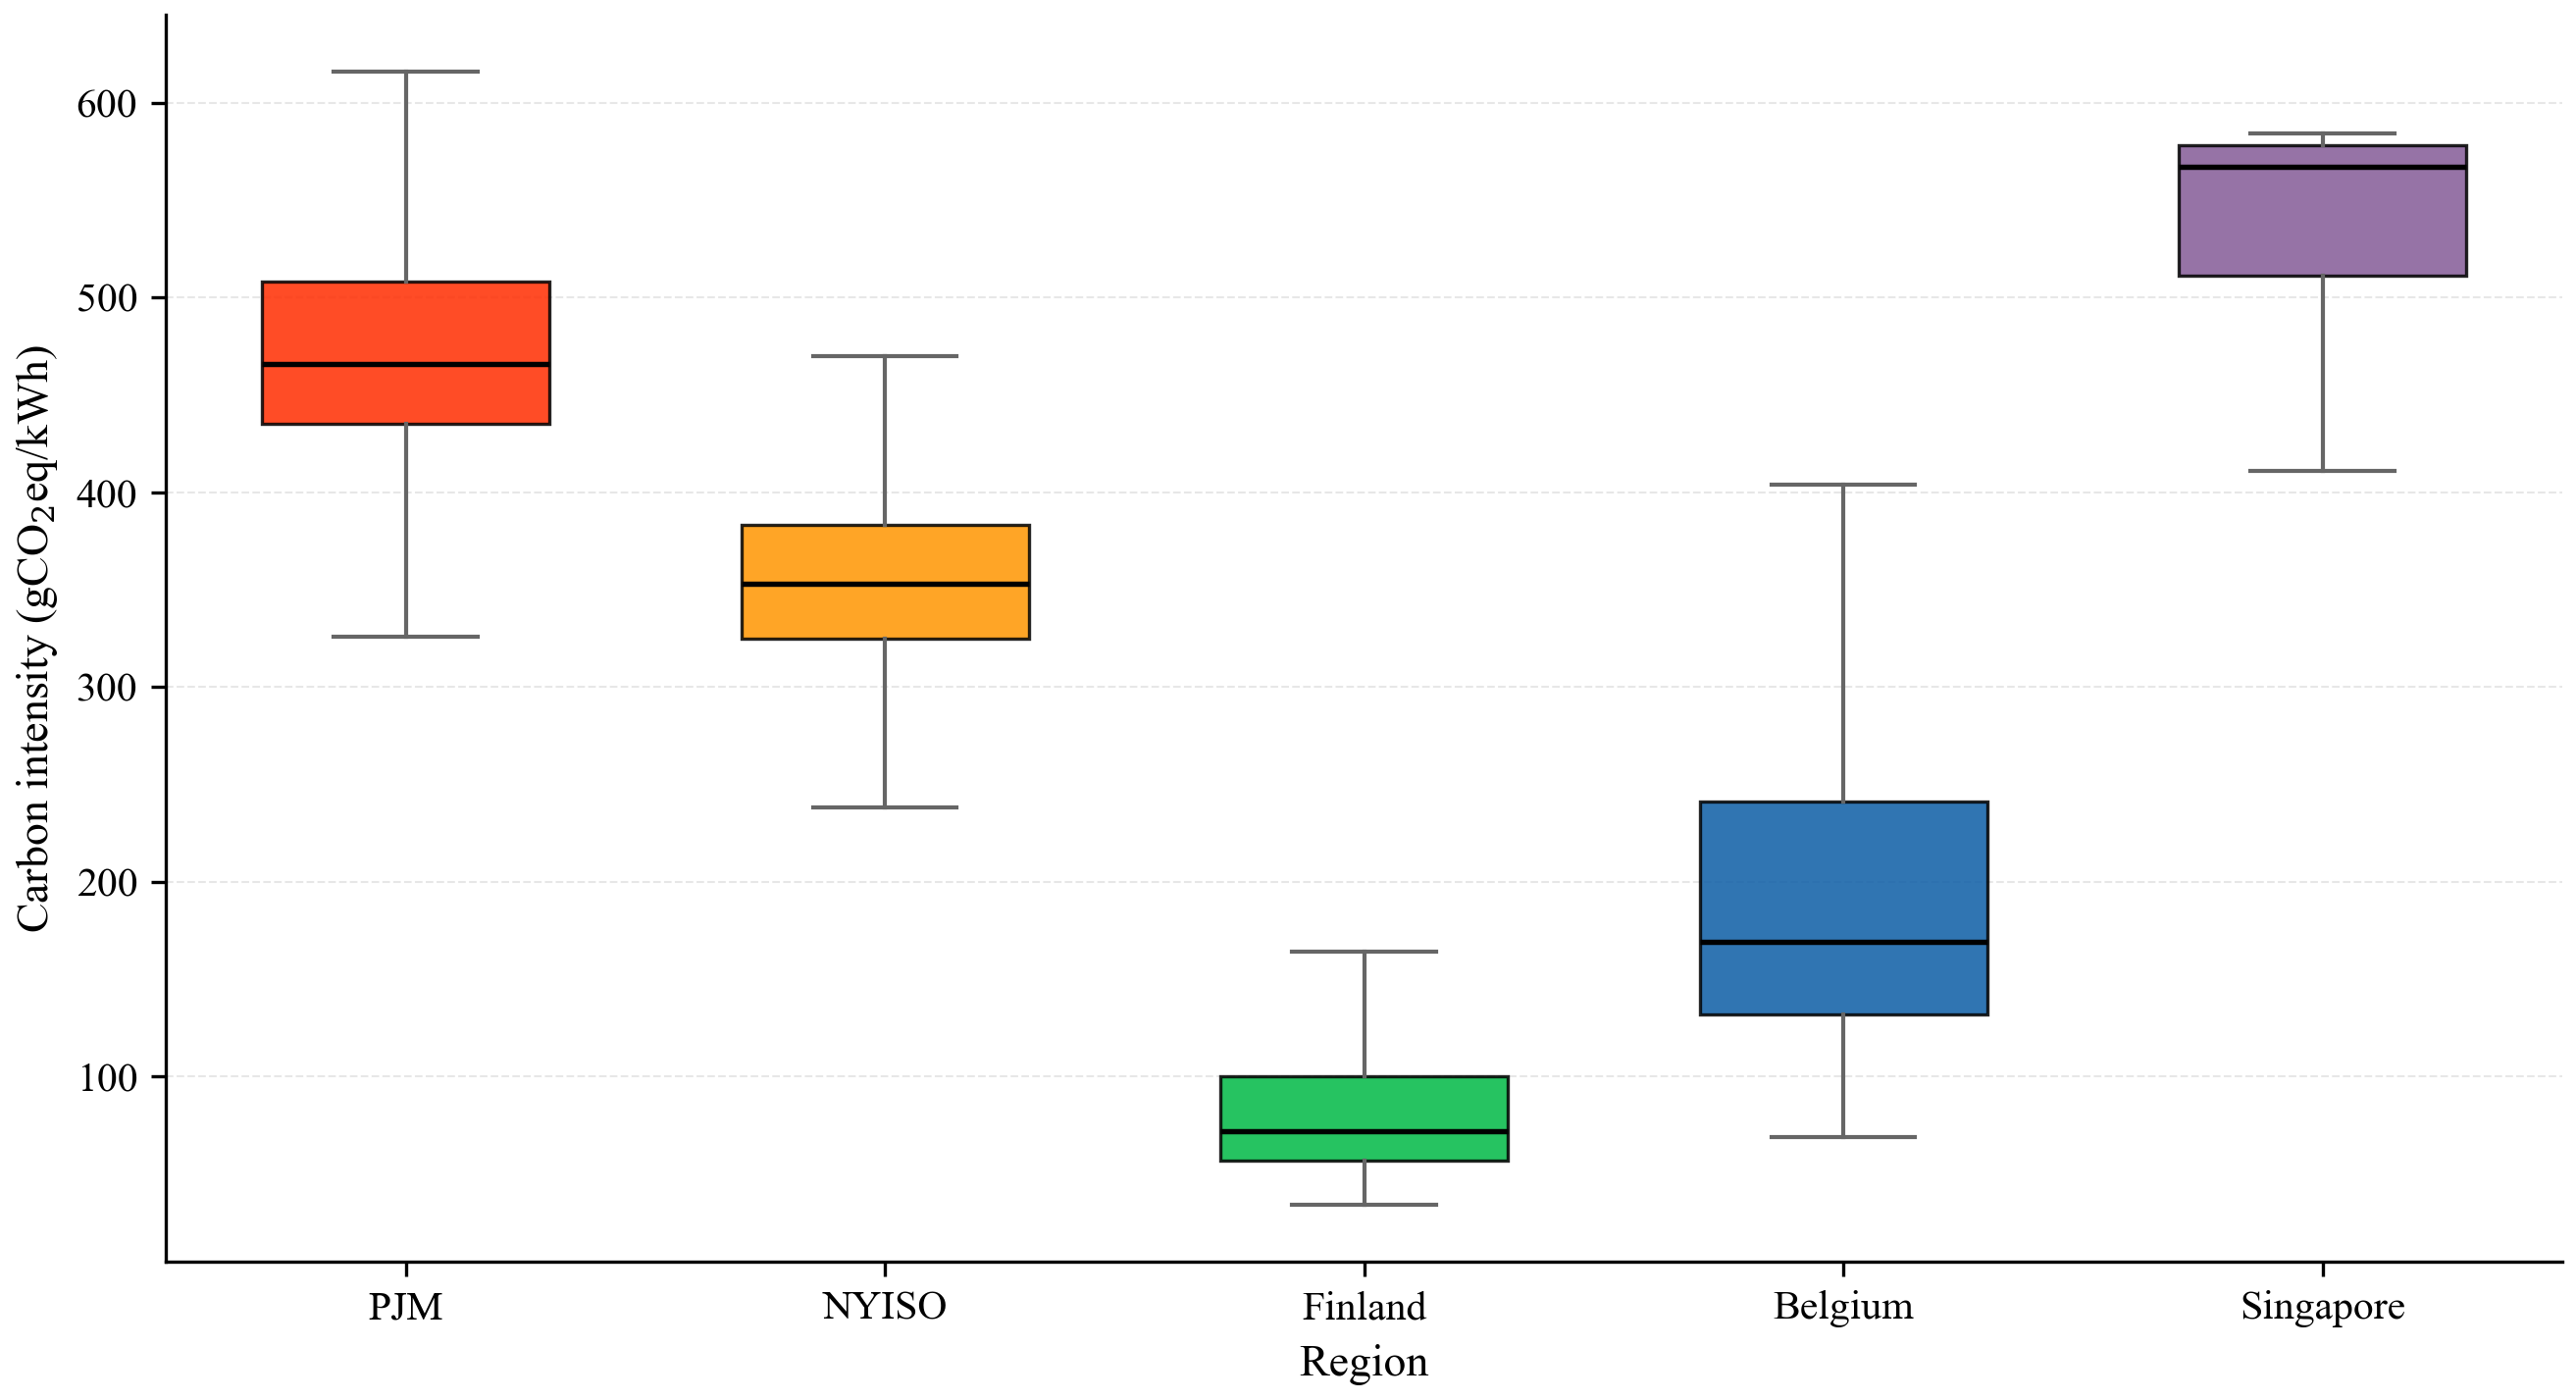
\includegraphics[width=\linewidth]{eda_ci_boxplot}
\fcap{Median CI differs by almost \textbf{7$\times$} (Finland $\sim$80 to Singapore $\sim$530\,gCO\textsubscript{2}eq/kWh).}
\vskip0.5ex
\hrule height0.4pt
\vskip0.5ex
\centering{\footnotesize\textbf{Per-region descriptive statistics}}
\vskip0.4ex
{\renewcommand{\arraystretch}{1.25}
\begin{tabularx}{\linewidth}{@{}l*{5}{>{\raggedleft\arraybackslash}X}@{}}
\toprule
\textbf{Region} & \textbf{CI} & \textbf{sd} & \textbf{range} & \textbf{CFE} & $\boldsymbol{R^2}$\\
\midrule
PJM       & 472 & 52 & 313--627 & 42.0 & 0.75\\
NYISO     & 354 & 44 & 215--499 & 51.1 & 0.77\\
Finland   &  83 & 35 &  34--285 & 94.0 & 0.97\\
Belgium   & 191 & 76 &  69--433 & 76.1 & 0.96\\
Singapore & 533 & 60 & 391--584 &  2.7 & 0.06\\
\bottomrule
\end{tabularx}}
\fcap{CI and its standard deviation and range in gCO\textsubscript{2}eq/kWh; CFE in \%; $R^2$ of CI on CFE.}
\end{block}
\vfill
\begin{block}{\sn{4} Spatial Decorrelation Enables Routing}
\centering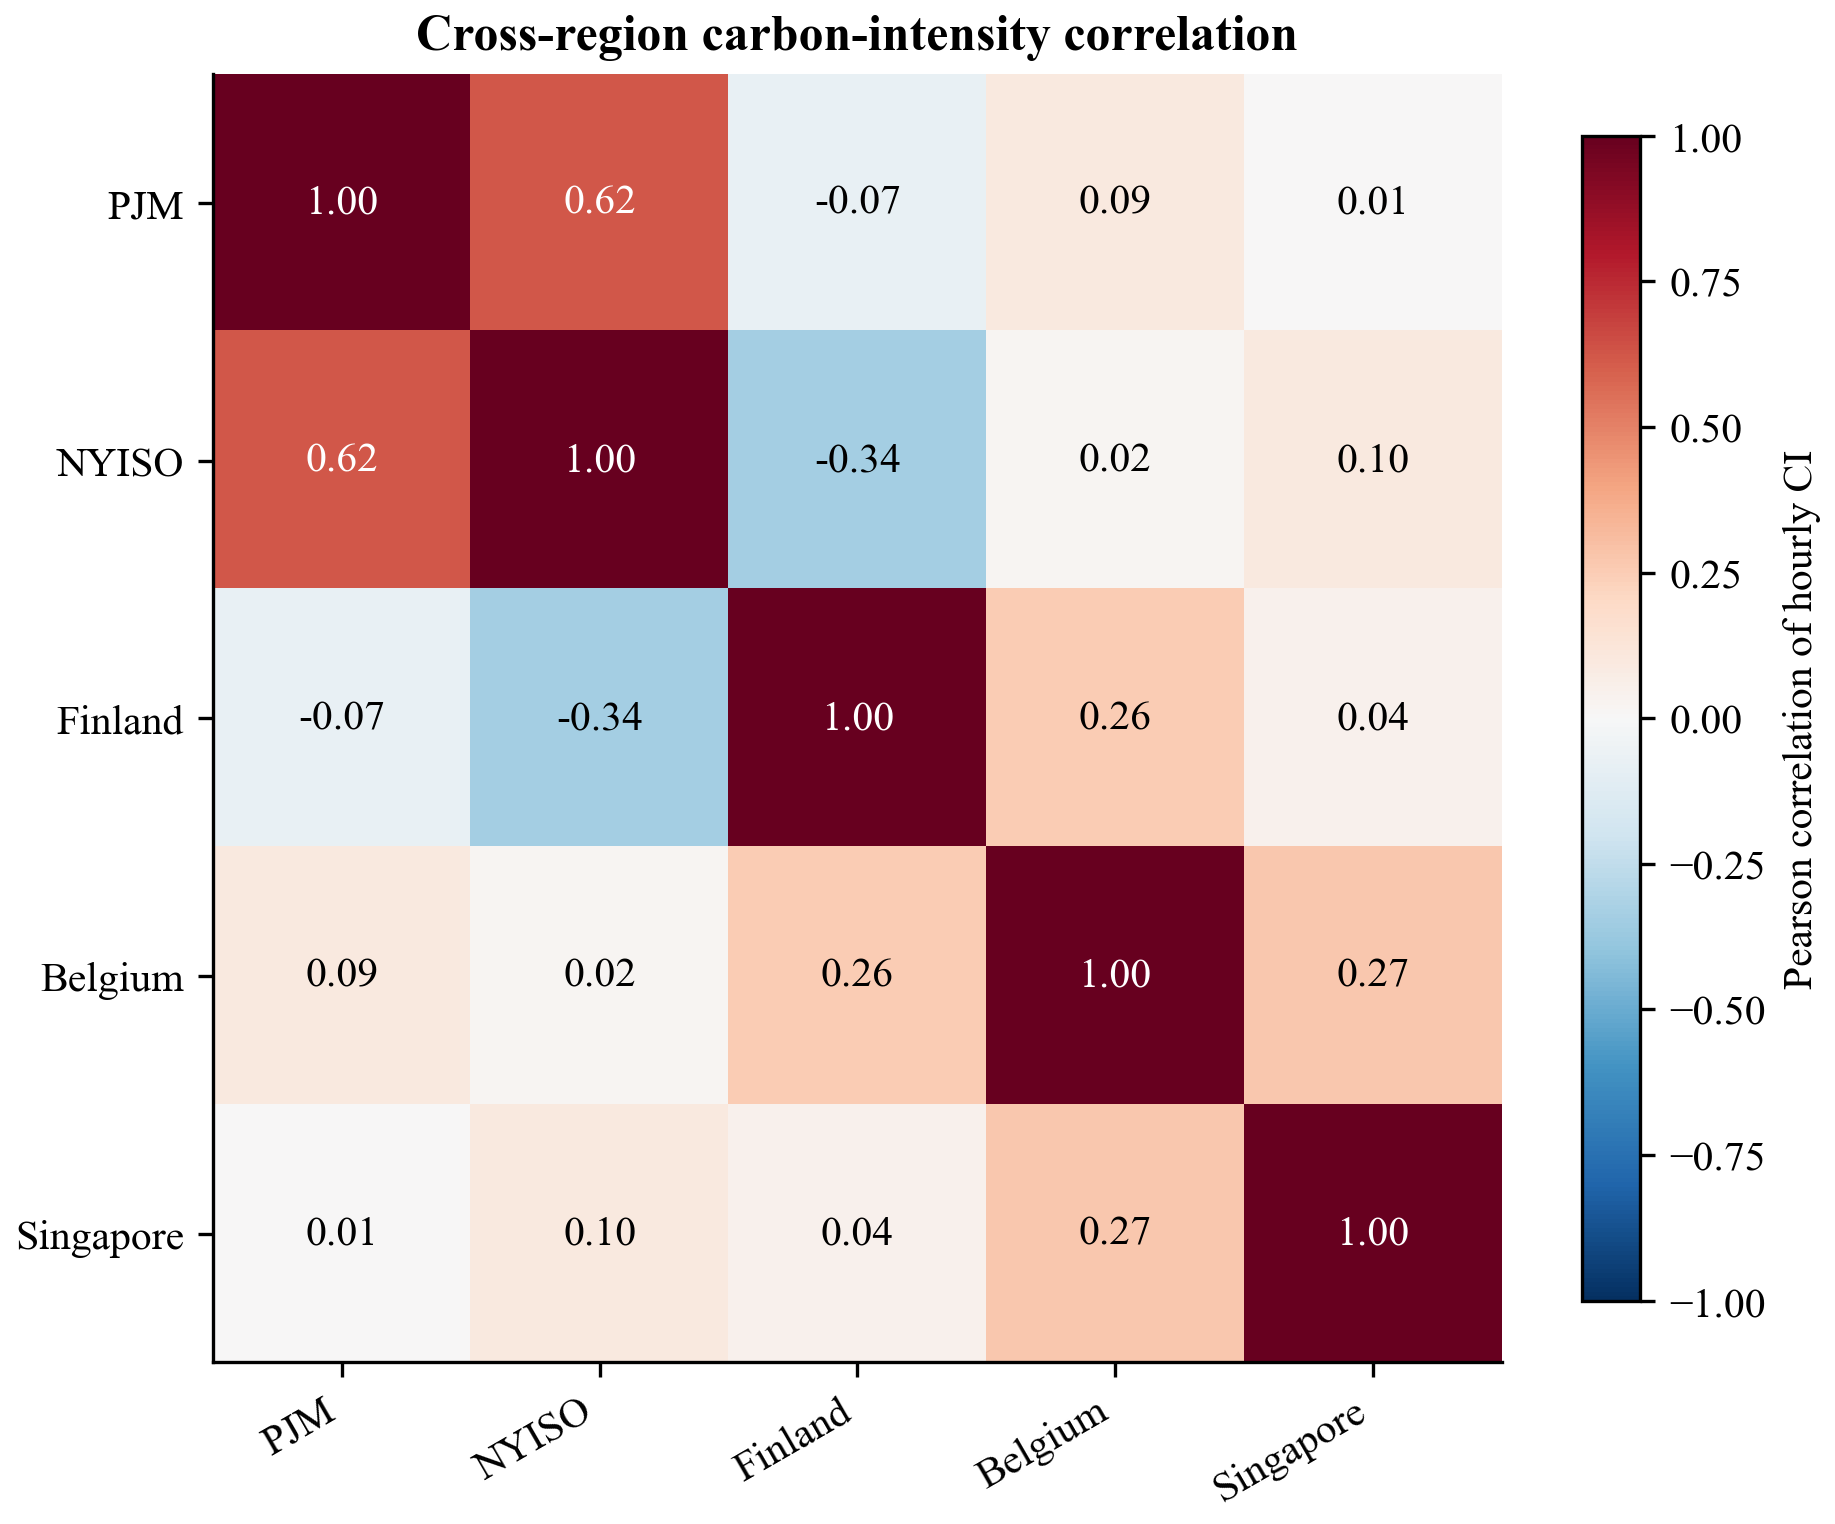
\includegraphics[width=0.8\linewidth]{eda_ci_correlation}
\fcap{Off-diagonal CI correlations are near zero or negative: when one grid is dirty, another is usually clean --- the structural precondition for spatial routing.}
\end{block}
\vfill
\begin{block}{\sn{5} Diurnal Structure of Carbon}
\centering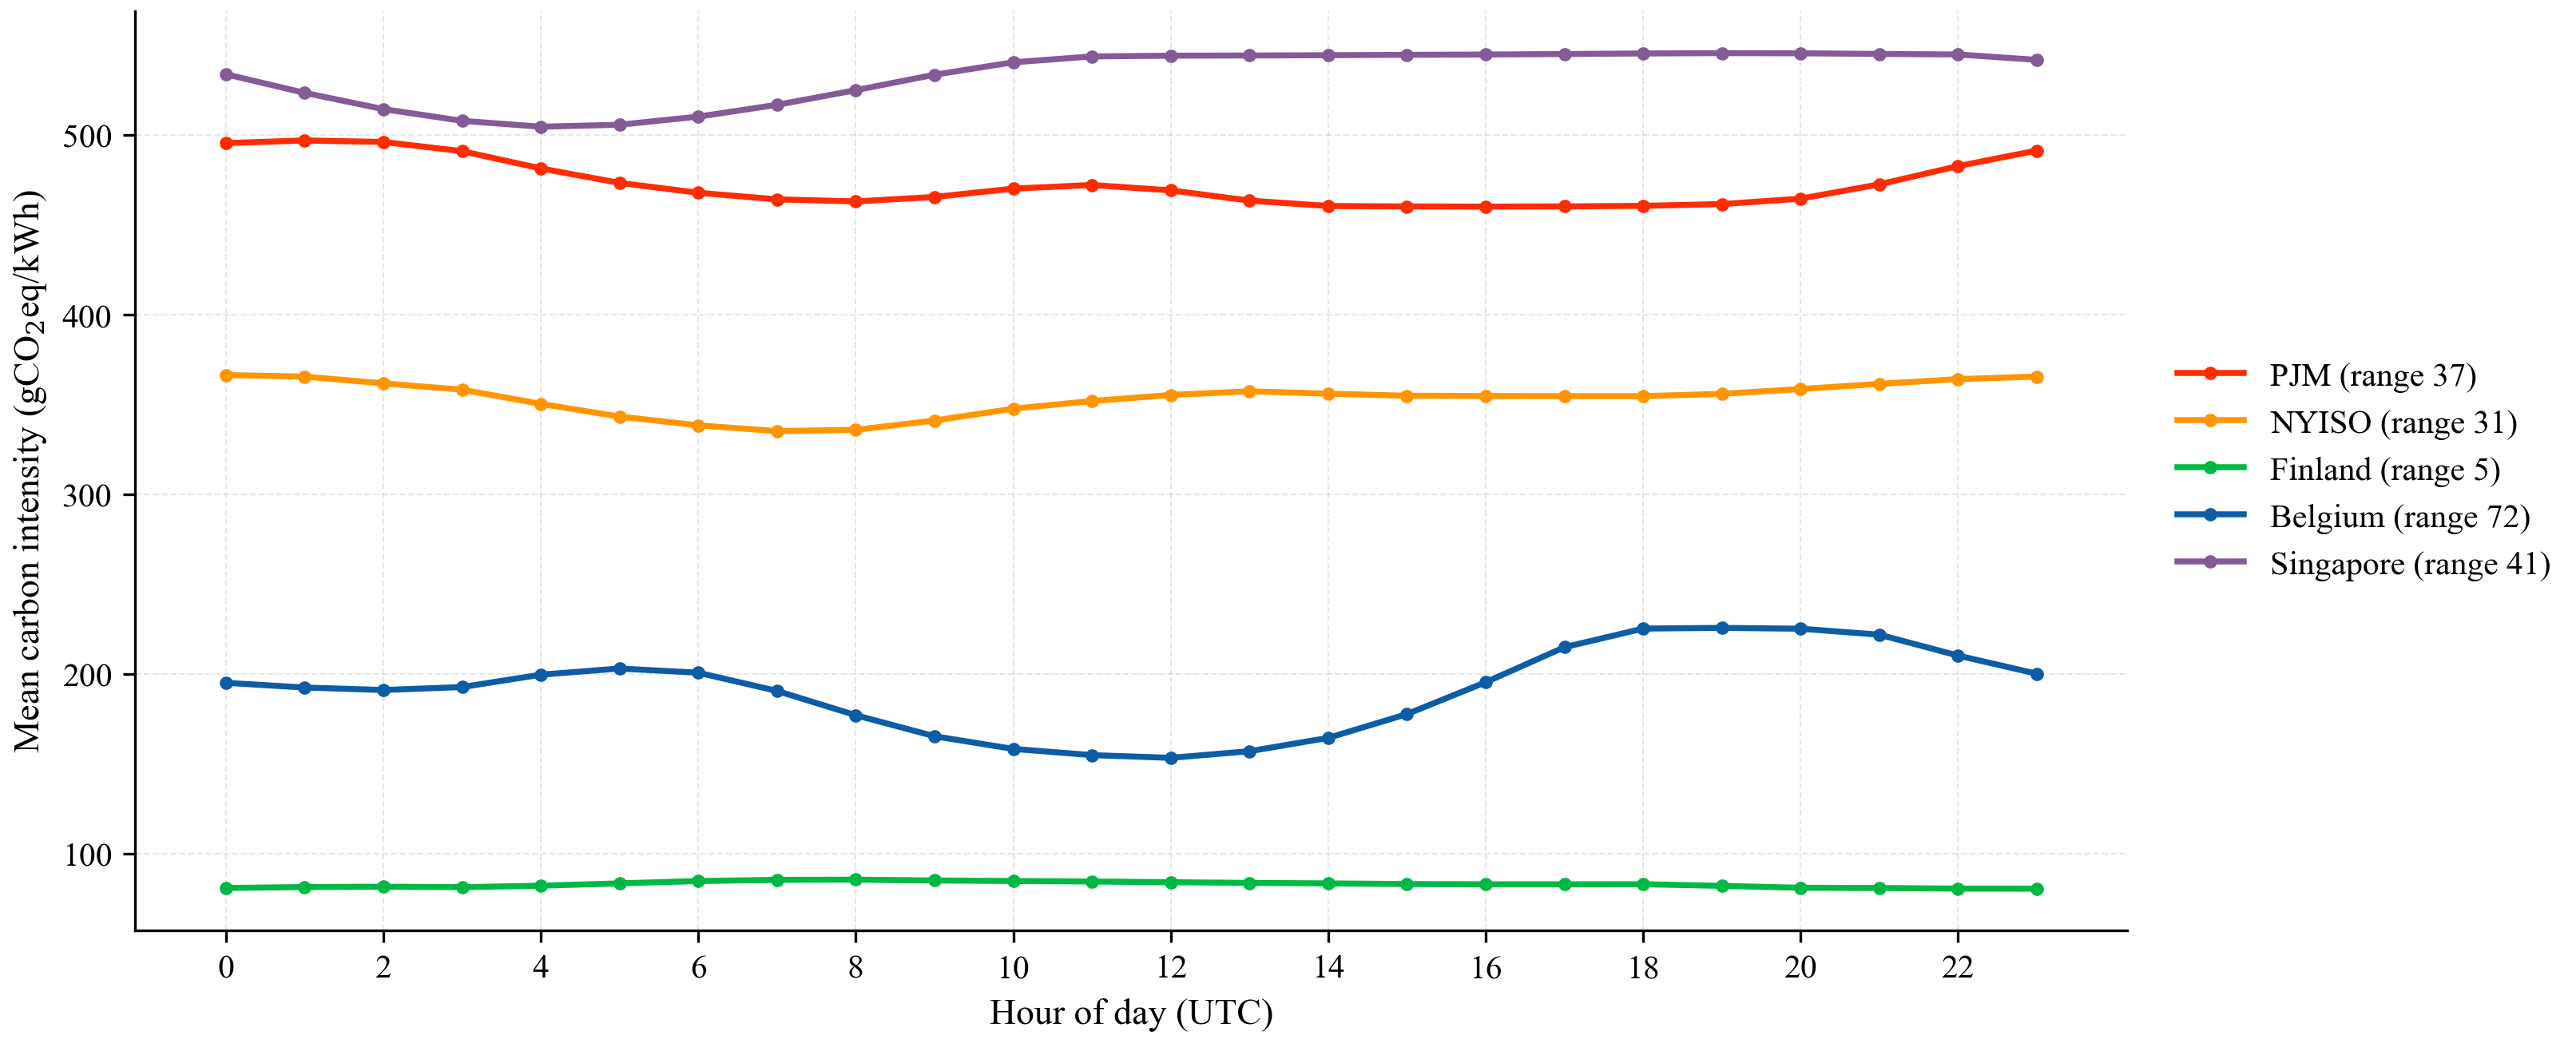
\includegraphics[width=\linewidth]{eda_diurnal}
\fcap{Intra-day CI range is largest in Belgium (midday solar) and smallest in Finland --- yet Finland is the most variable region overall on a multi-day basis.}
\end{block}

\end{minipage}
\end{column}

% =========================== COLUMN 2 ===========================
\begin{column}{\colw}
\begin{minipage}[t][\colht]{\linewidth}

\begin{block}{\sn{6} Seasonal Structure of Carbon}
\centering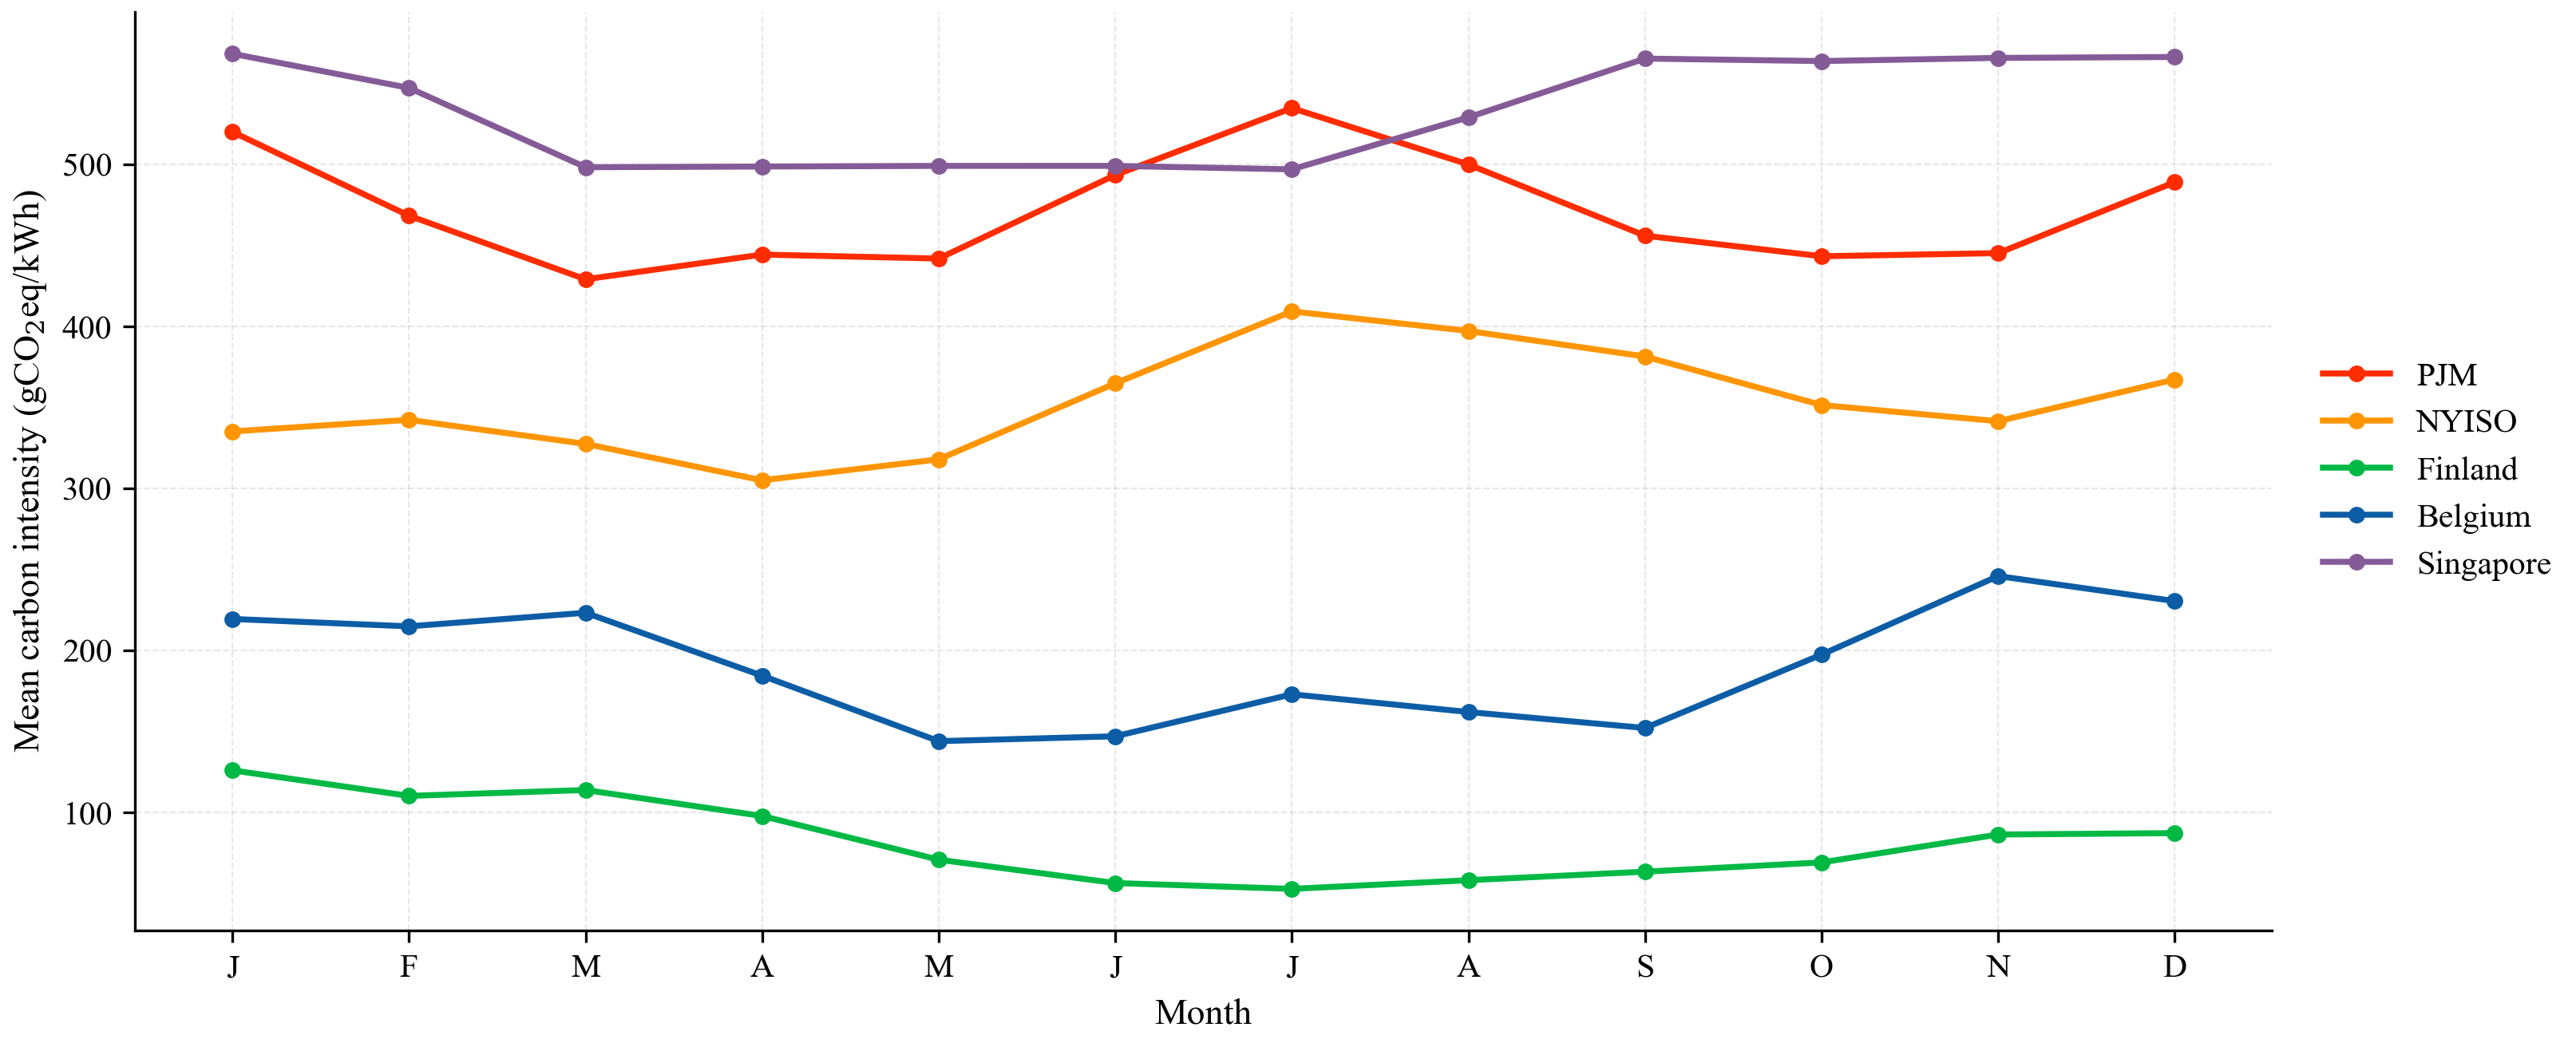
\includegraphics[width=\linewidth]{eda_monthly}
\fcap{Finland and Belgium show seasonal troughs as renewables peak; PJM and Singapore stay high year-round. Seasonal swings exceed diurnal ones in clean grids, motivating the two-year horizon.}
\end{block}
\vfill
\begin{block}{\sn{7} Why CFE? \ CI vs.\ Carbon-Free Fraction}
\centering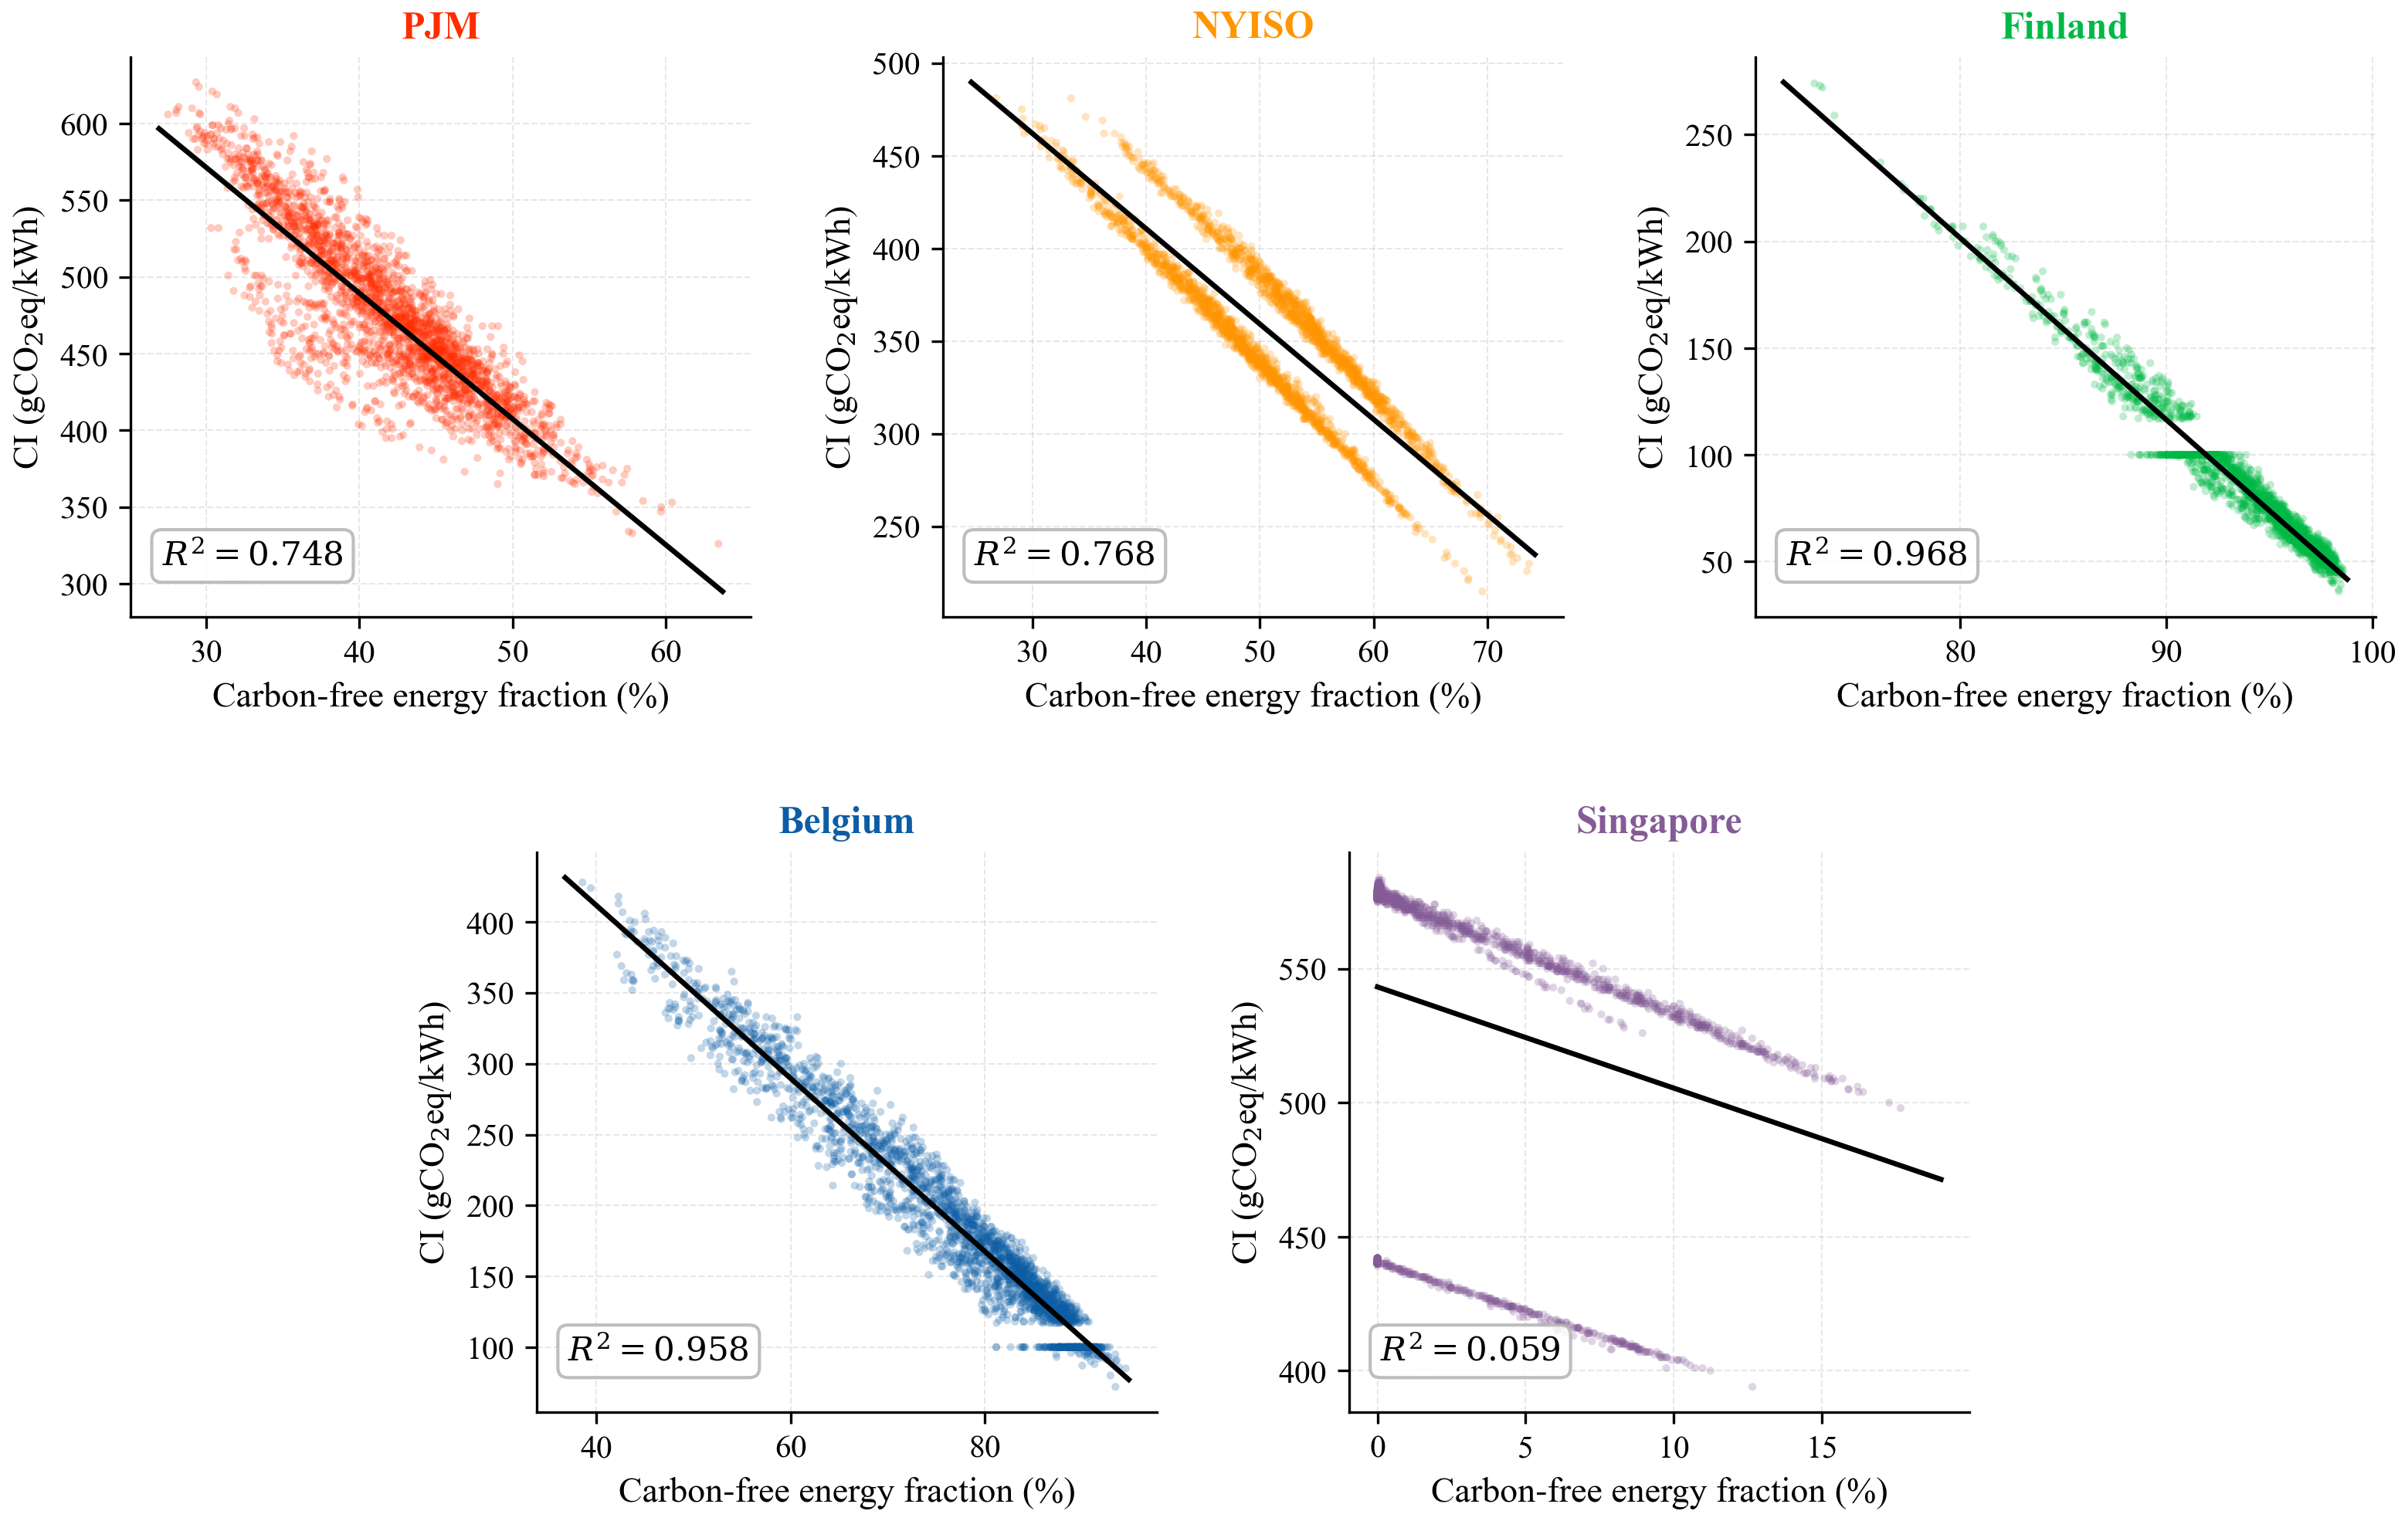
\includegraphics[width=\linewidth]{eda_ci_cfe_regression}
\fcap{CFE explains most of the variation in CI ($R^2$ up to 0.97), except in gas-dominated Singapore --- supporting CFE as a cleanliness signal alongside CI.}
\end{block}
\vfill
\begin{block}{\sn{8} Carbon-Free Supply Composition}
\centering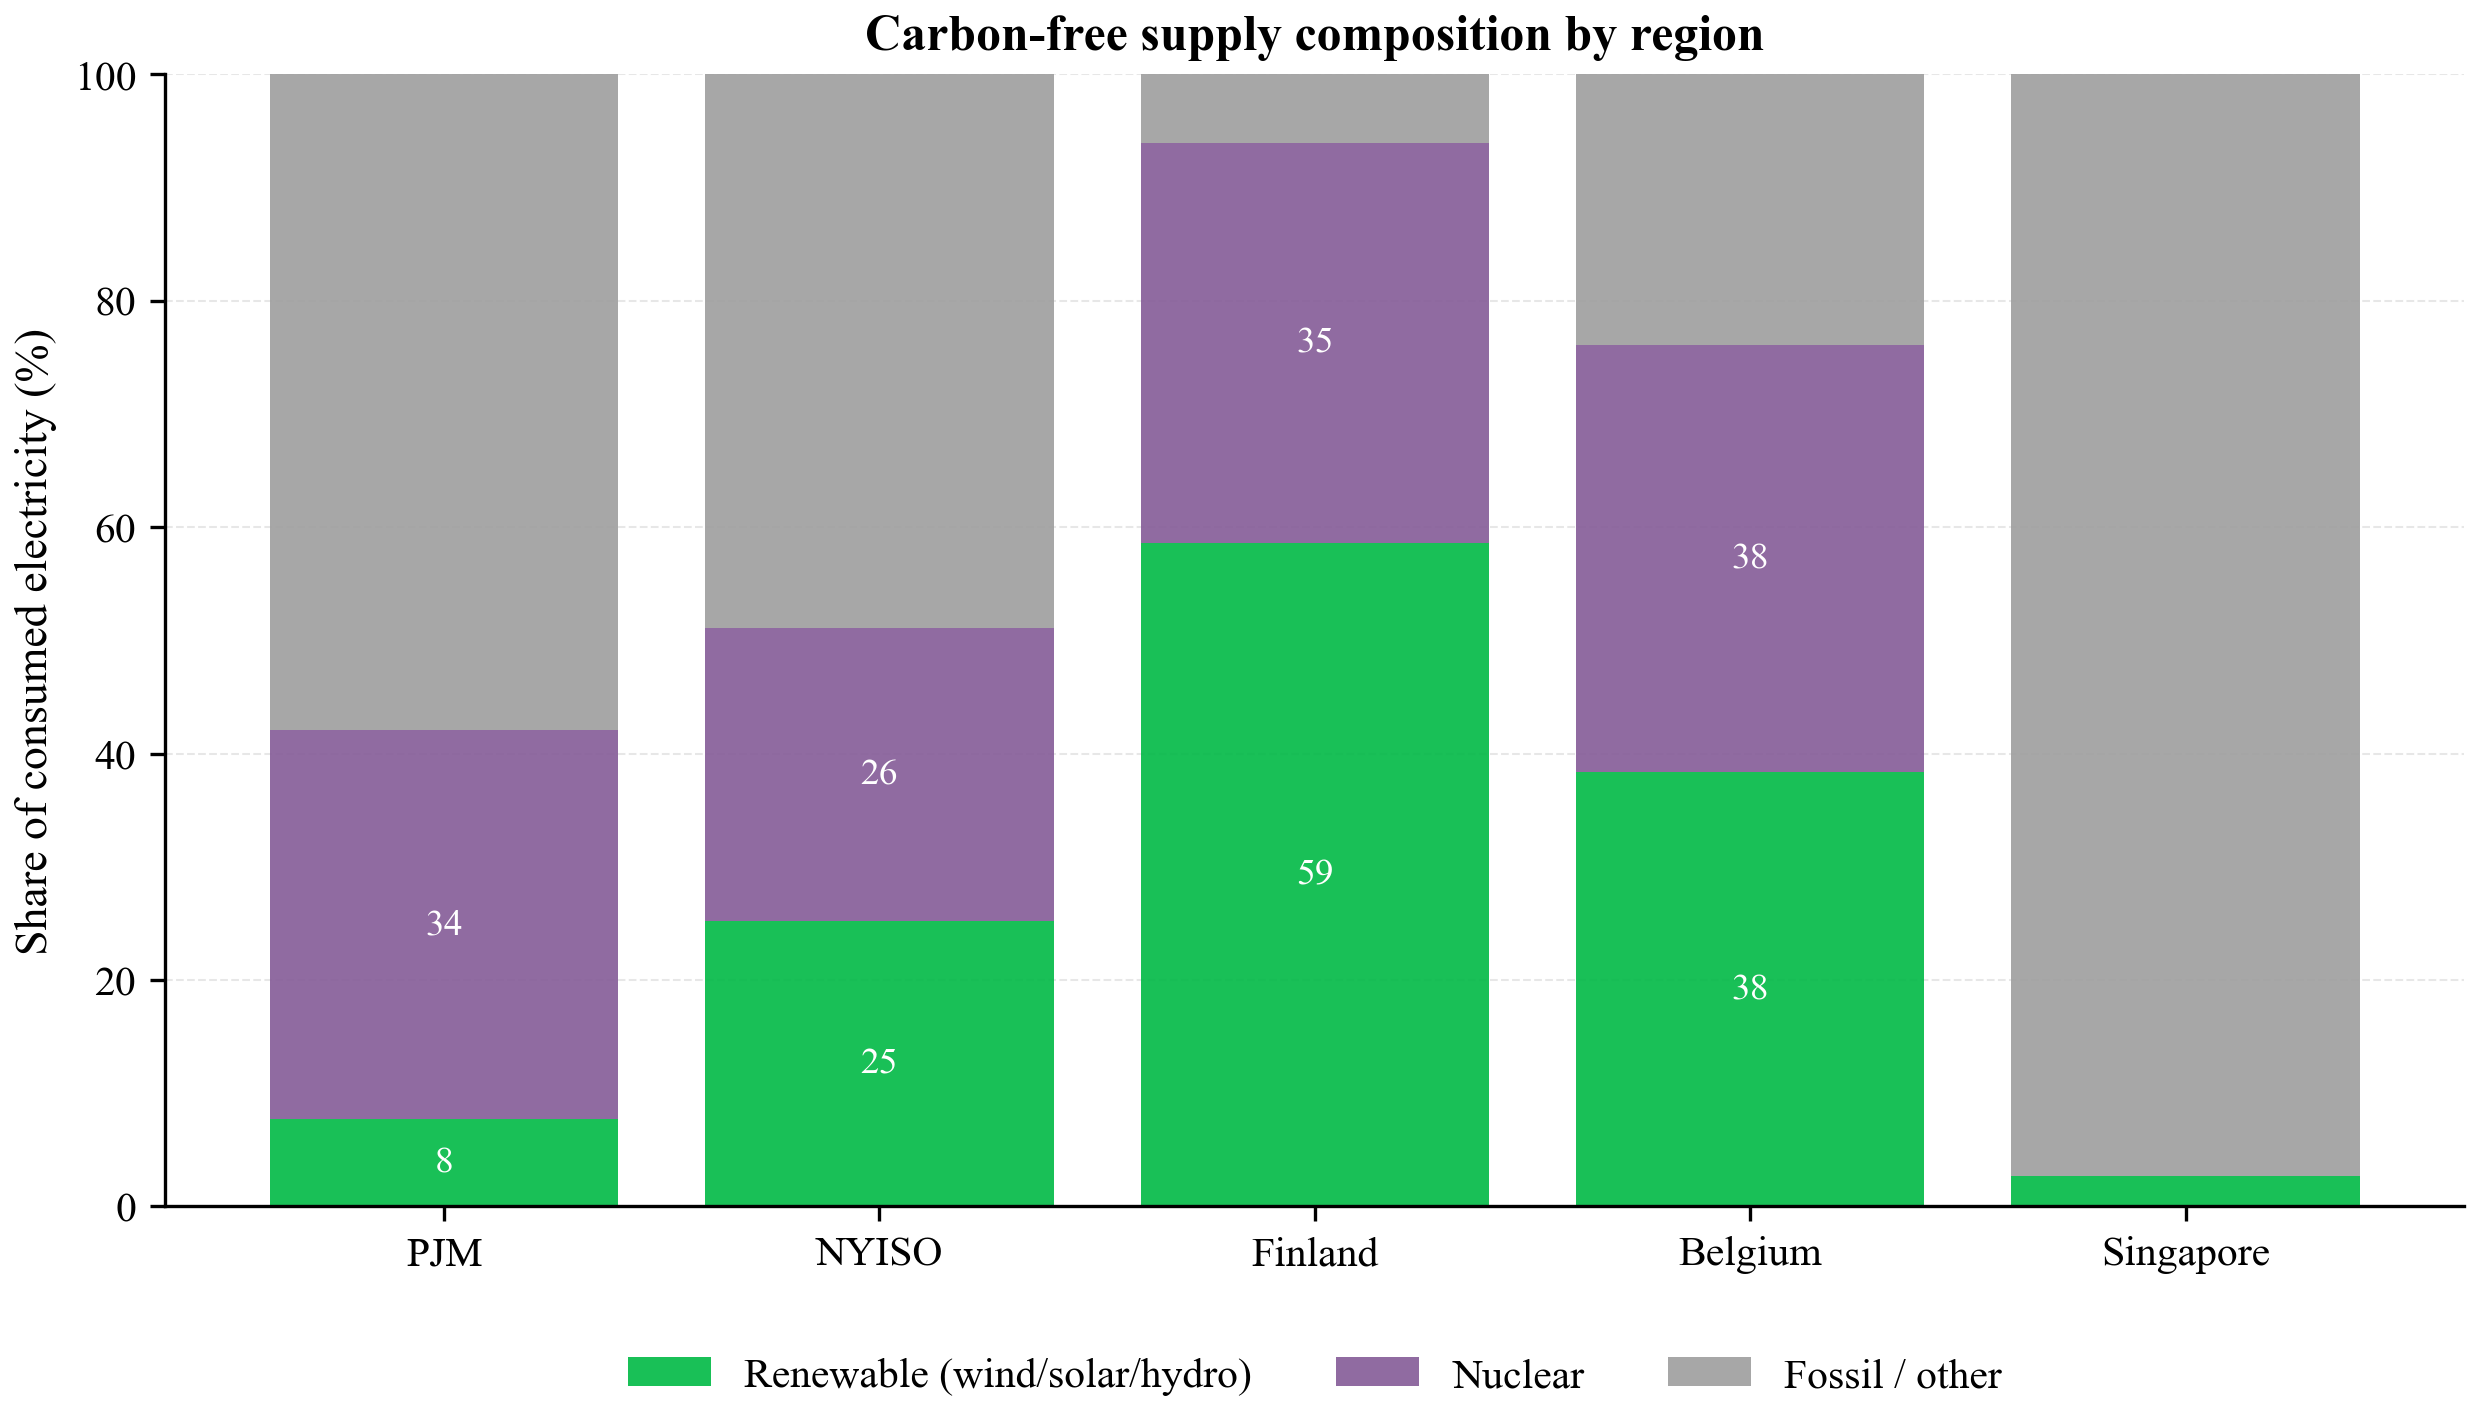
\includegraphics[width=\linewidth]{eda_cfe_composition}
\fcap{PJM and NYISO reach much of their carbon-free fraction through \emph{nuclear}, not renewables --- why a renewables-only signal would misrepresent them and CFE is used instead.}
\end{block}
\vfill
\begin{block}{\sn{9} CFE Signal: Cross-Validation}
\centering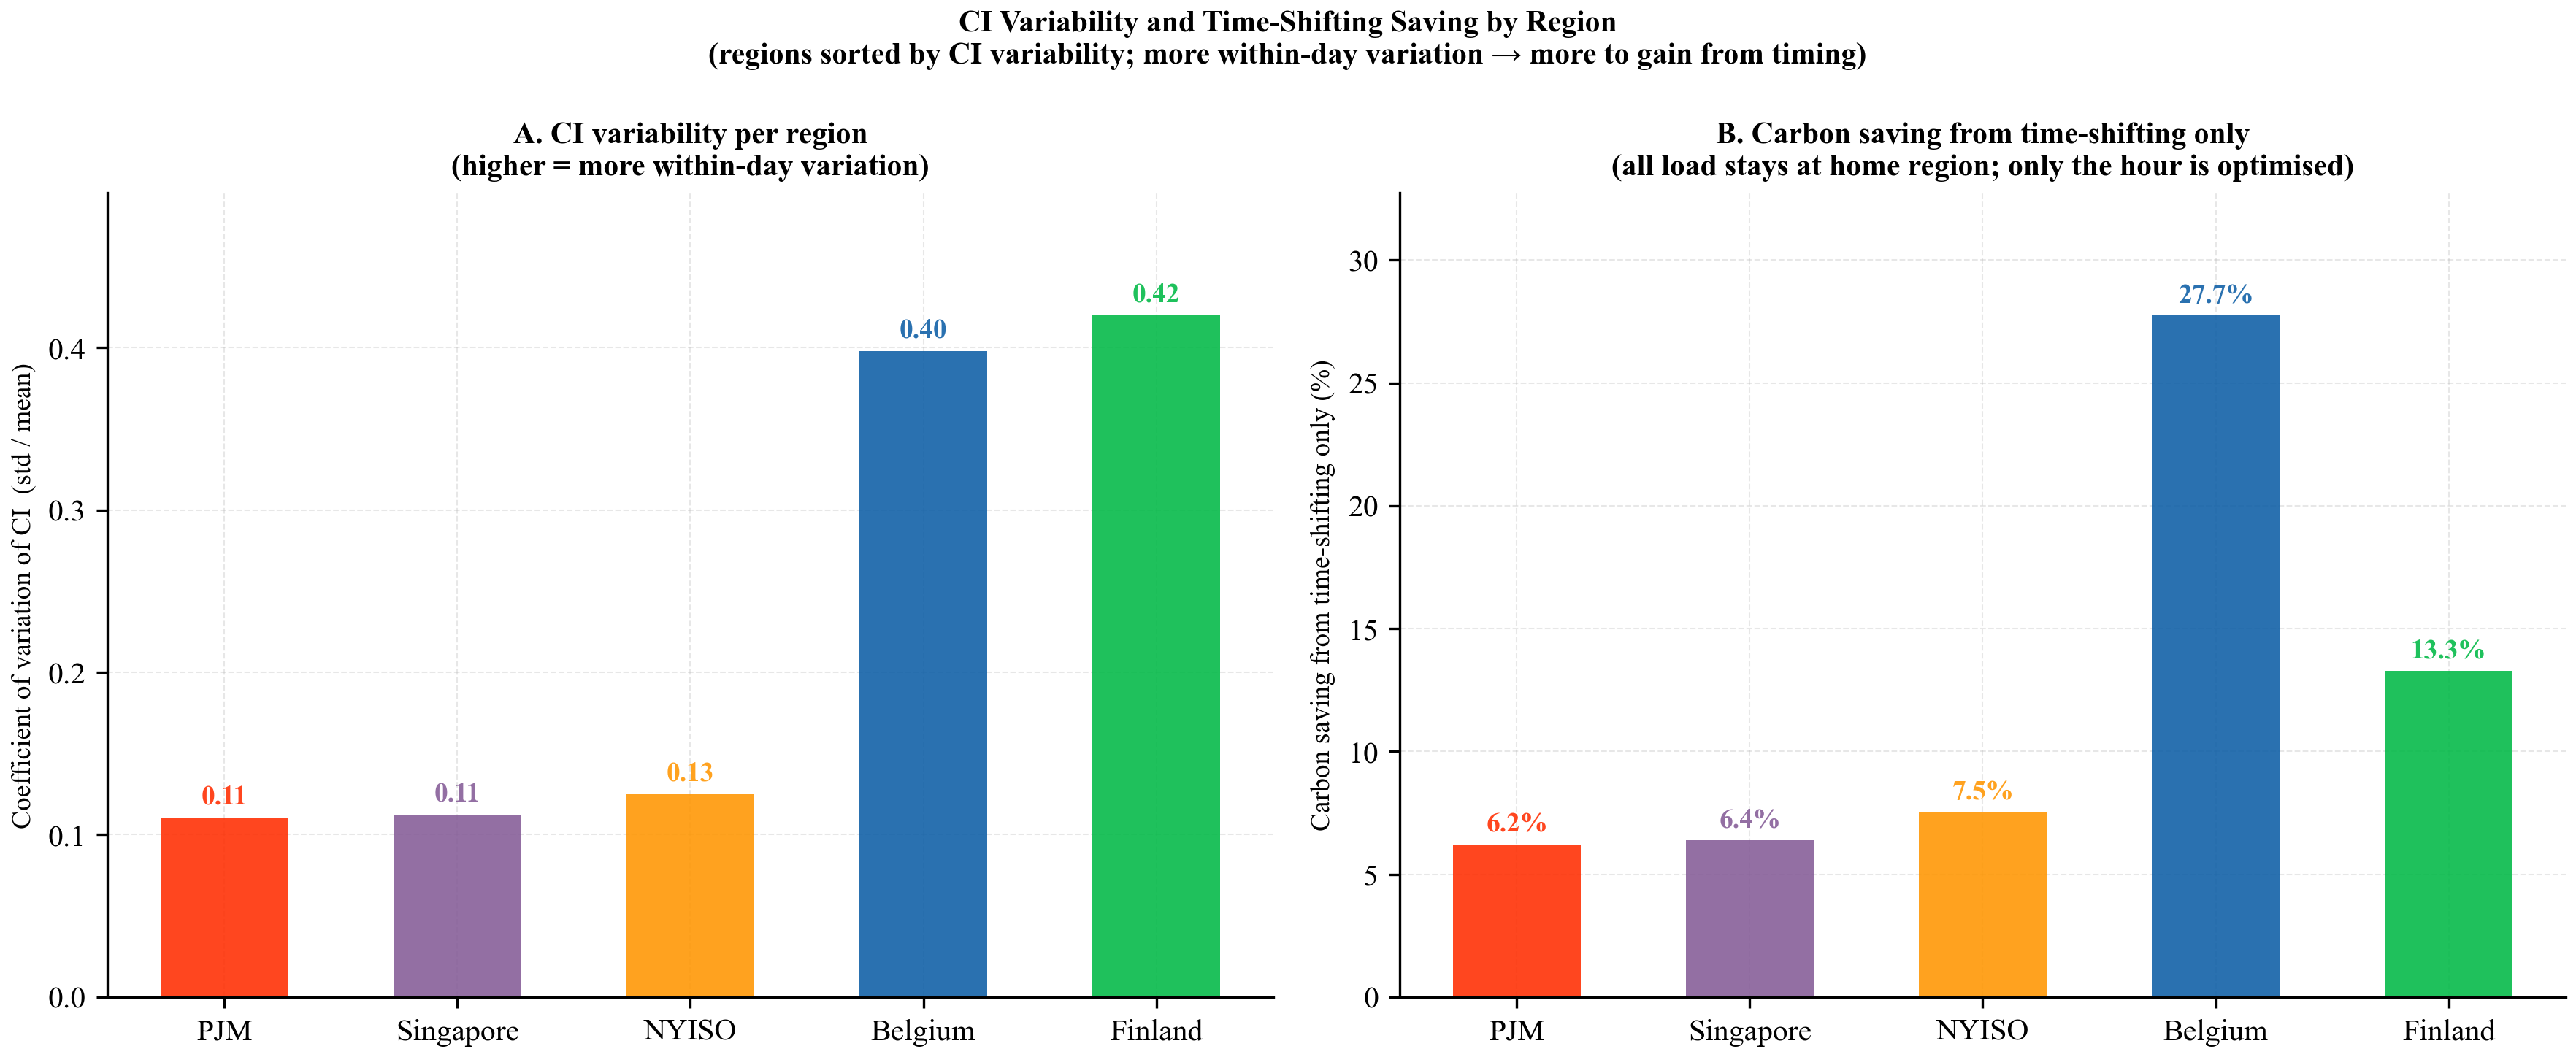
\includegraphics[width=\linewidth]{cv_regression}
\fcap{Five-fold cross-validation of the CI--CFE relationship confirms the signal generalises out-of-sample in every region except gas-fired Singapore.}
\end{block}
\vfill
\begin{block}{\sn{10} Validation}
\centering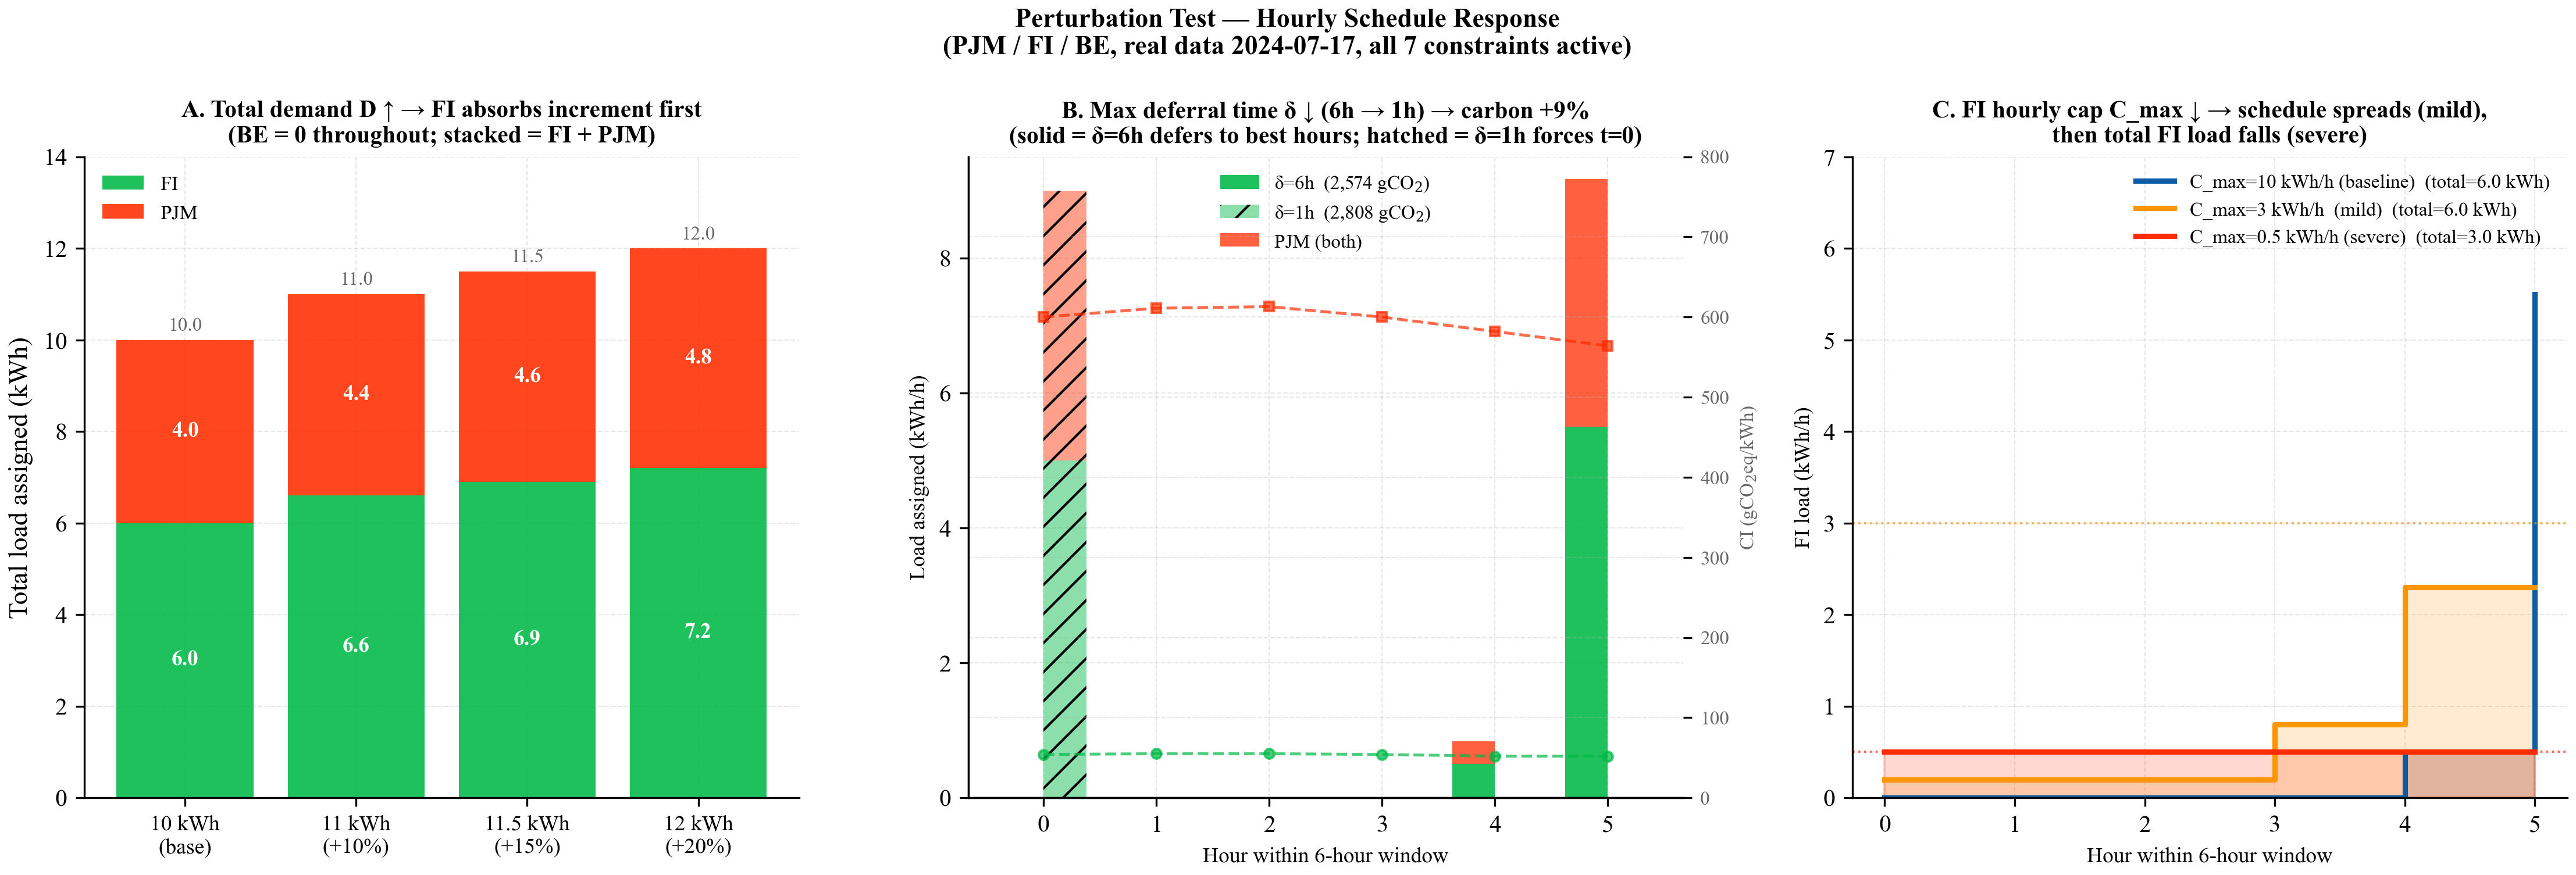
\includegraphics[width=0.94\linewidth]{perturbation_test}
\fcap{Behavioural perturbation test: the schedule reacts correctly to every input change (\textbf{13/13} checks pass).}
\vskip0.4ex
\centering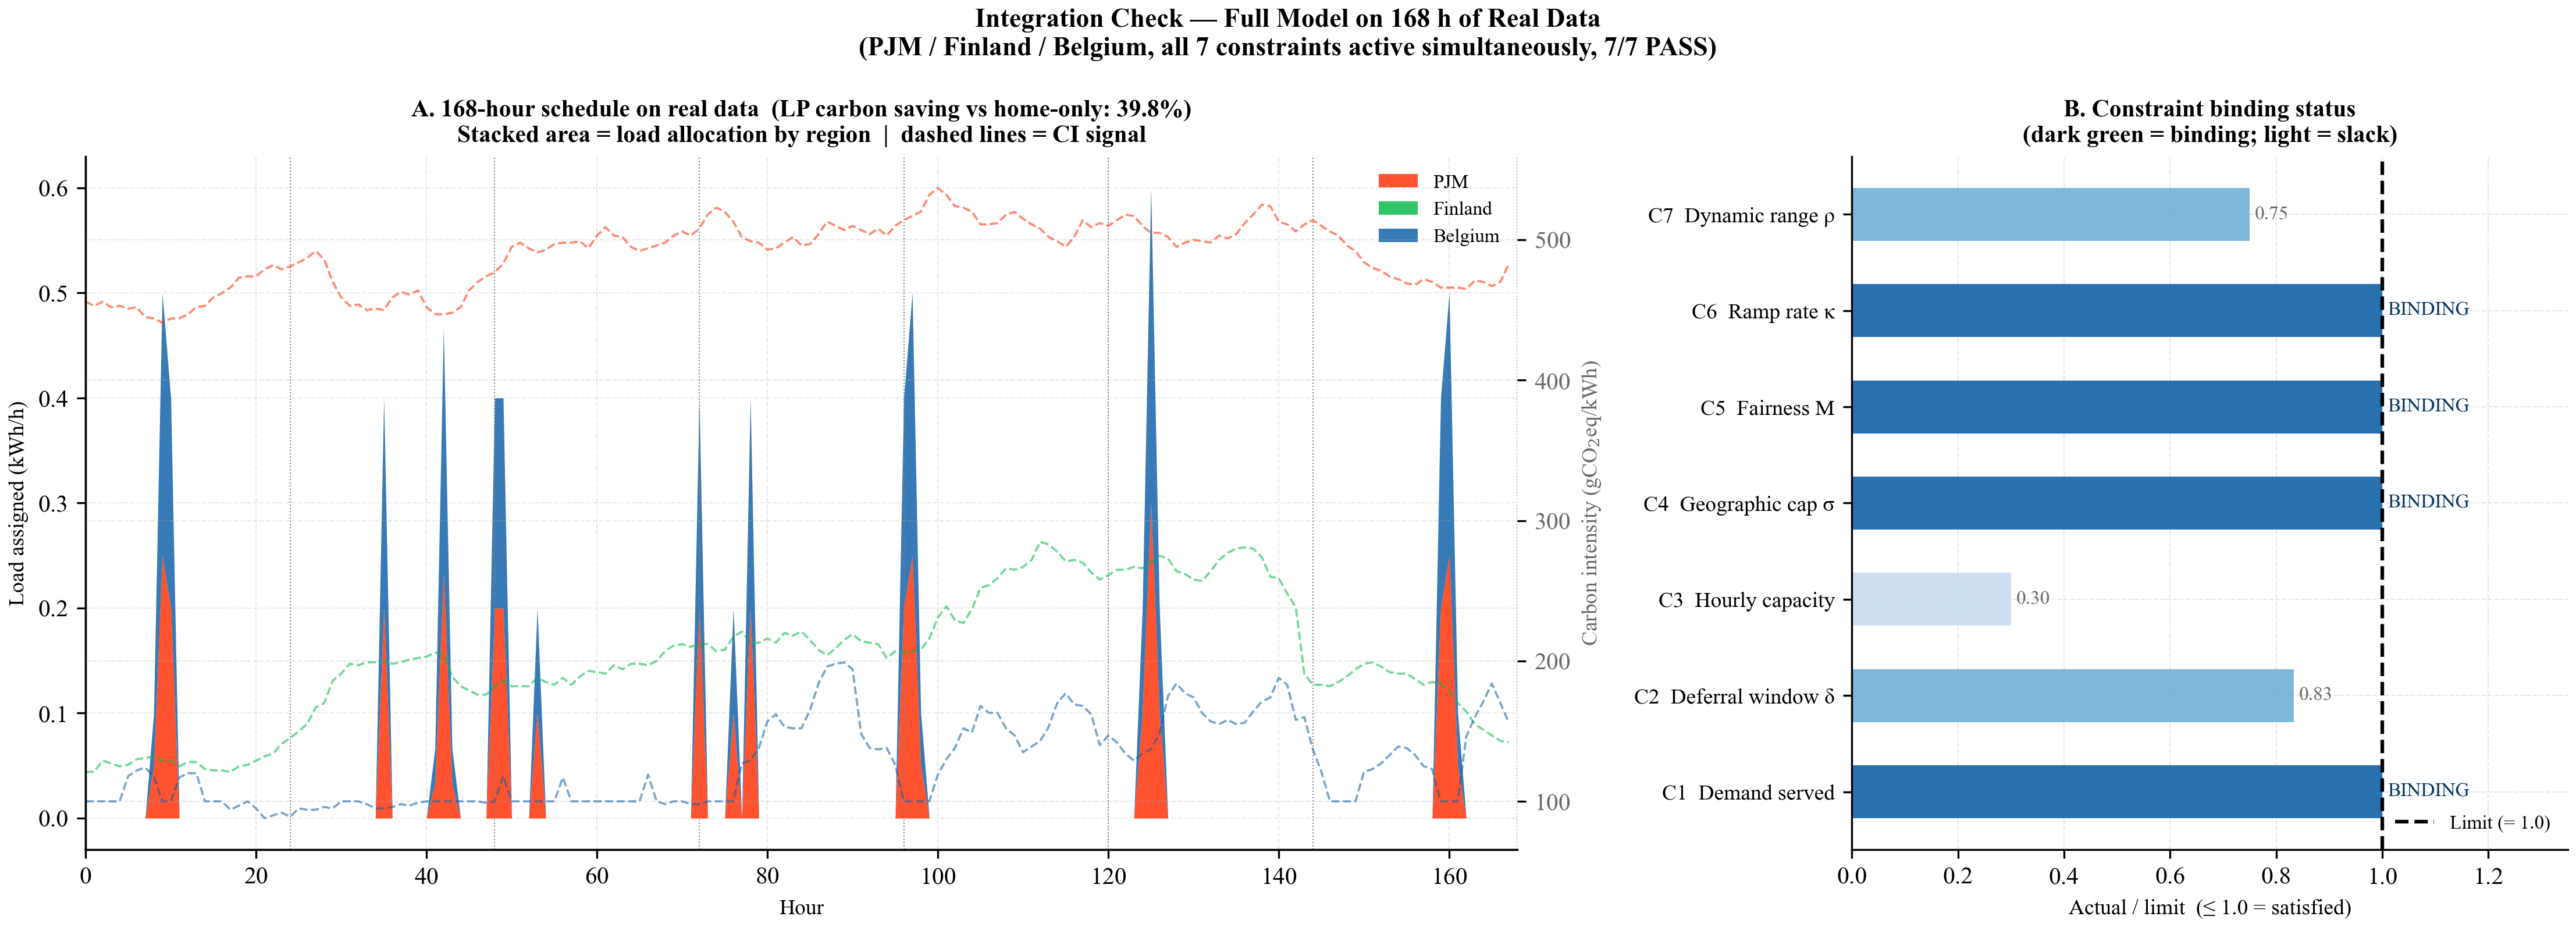
\includegraphics[width=0.78\linewidth]{integration_check}
\fcap{Integration check on 168\,h of real data: all \textbf{7/7} constraints hold; LP cuts carbon \textbf{39.8\%} vs.\ a home-only baseline.}
\end{block}

\end{minipage}
\end{column}

% =========================== COLUMN 3 ===========================
\begin{column}{\colw}
\begin{minipage}[t][\colht]{\linewidth}

\begin{block}{\sn{11} Schedule Illustration}
\centering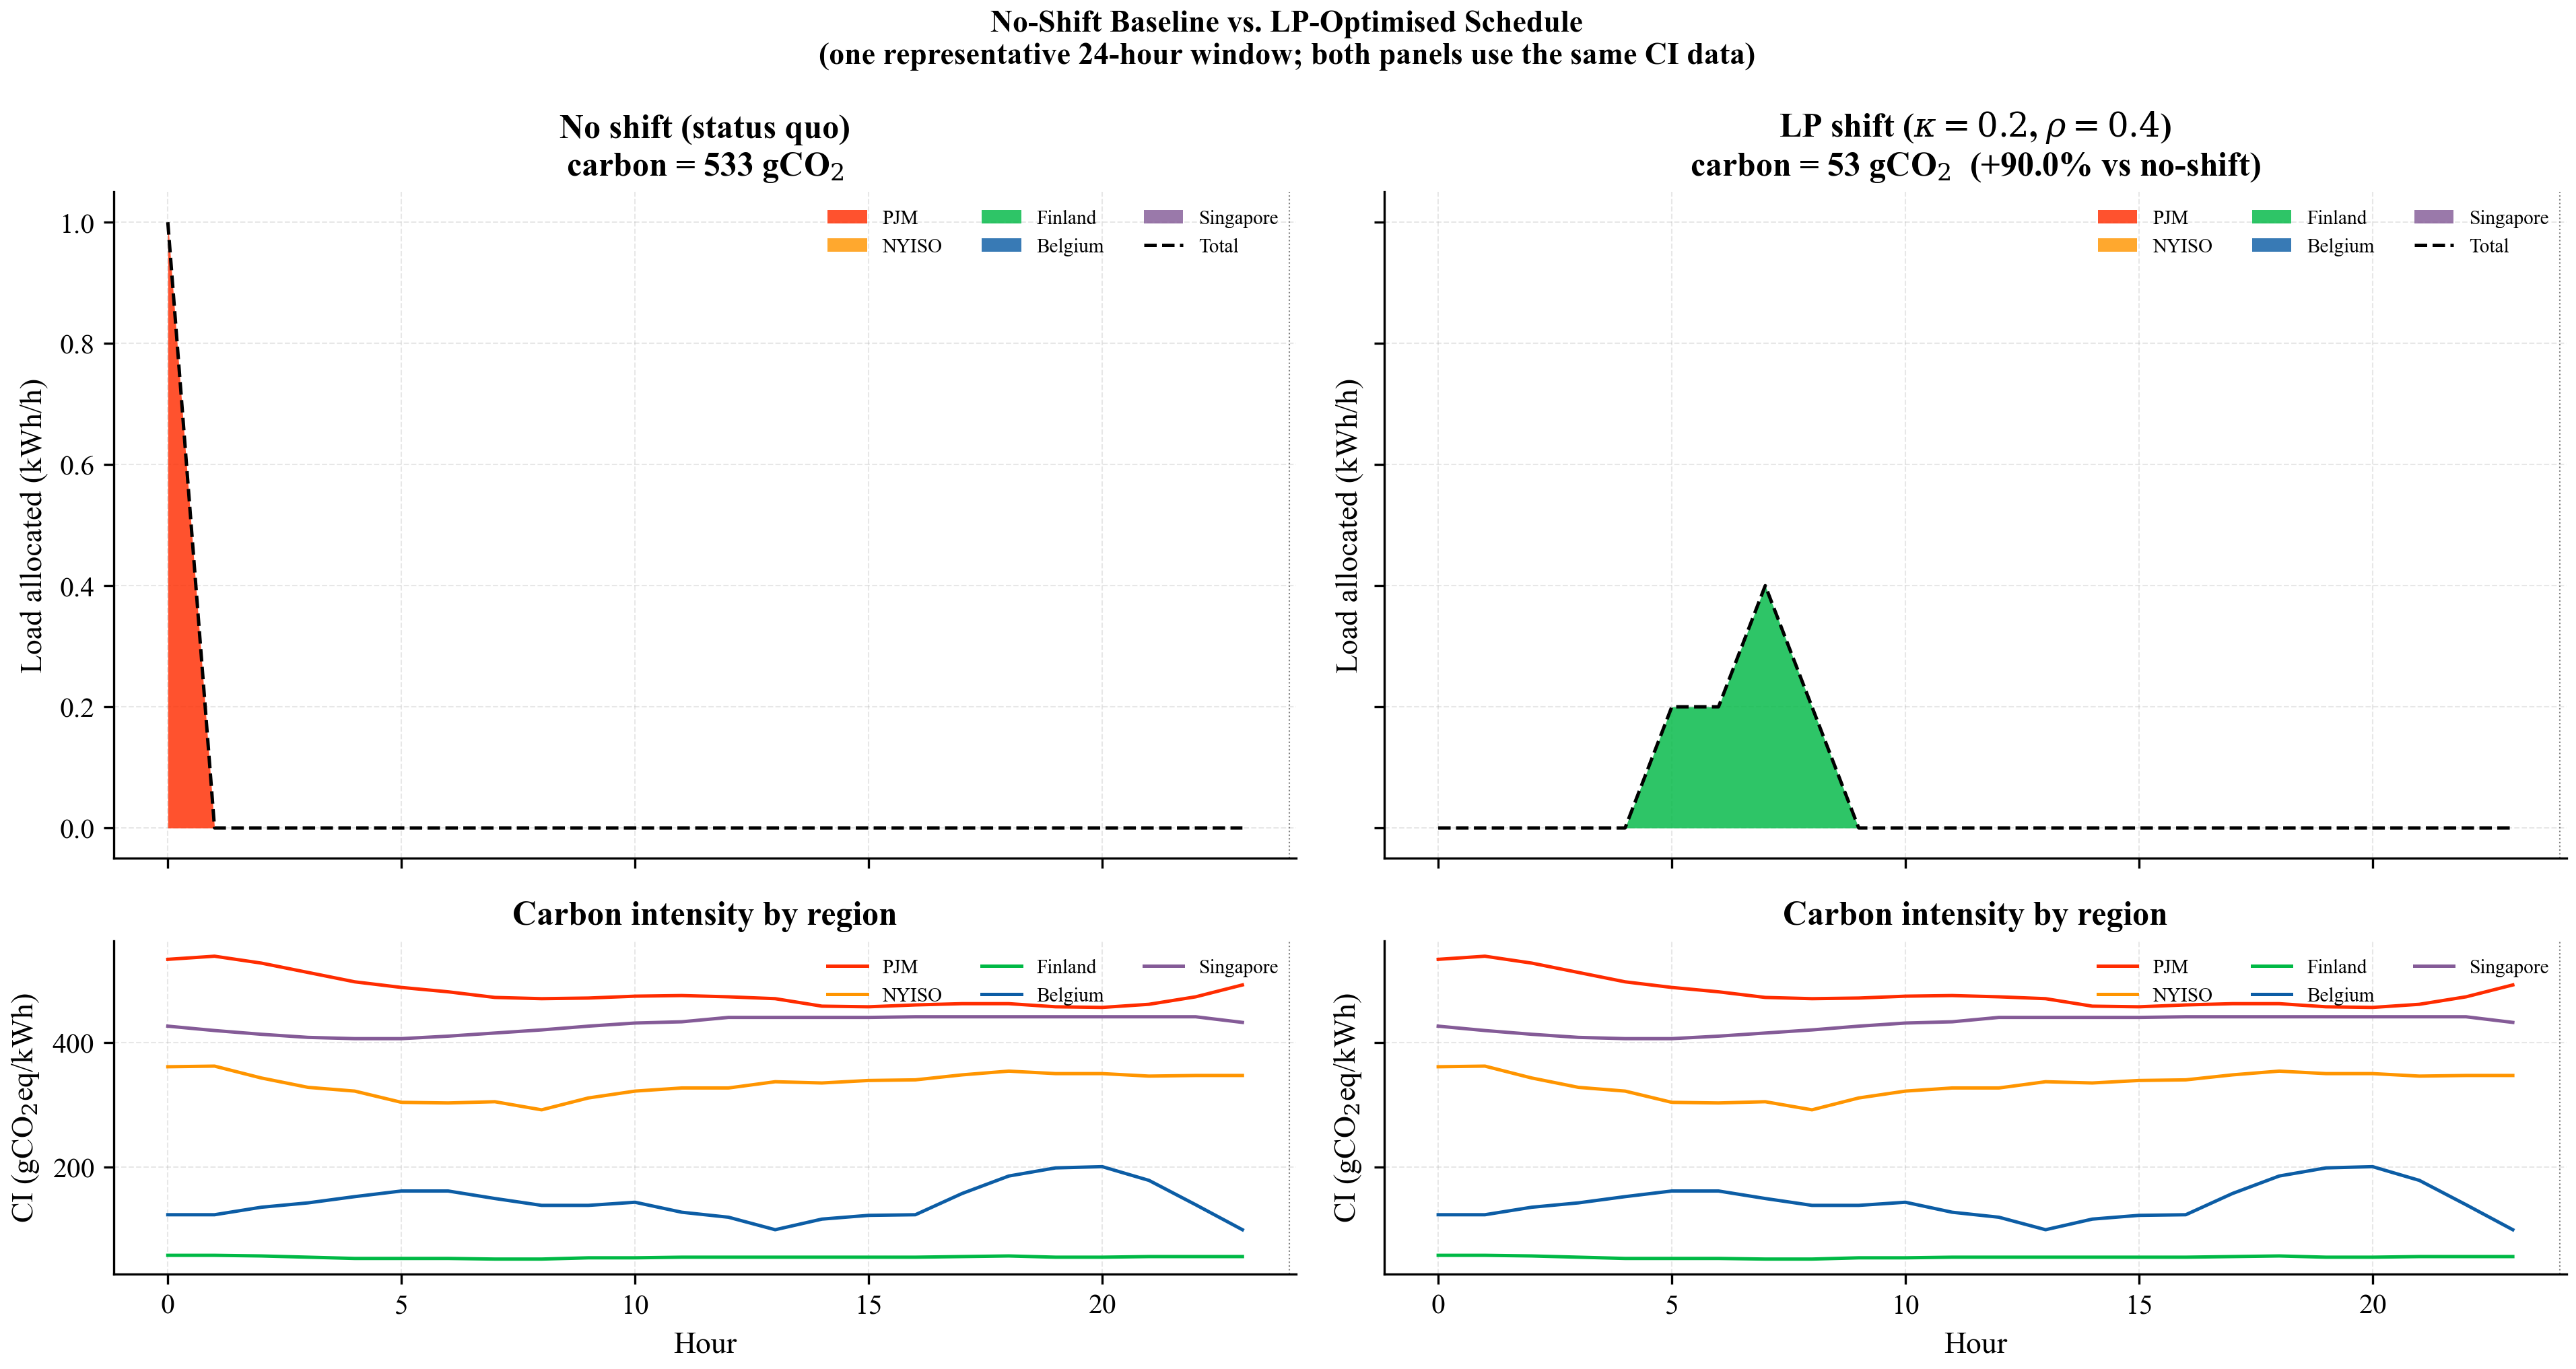
\includegraphics[width=\linewidth]{schedule_sample}
\fcap{One window: the LP routes the batch to Finland and spreads it across hours to respect the ramp limit, cutting window carbon from 533 to 53\,gCO\textsubscript{2}.}
\end{block}
\vfill
\begin{block}{\sn{12} Geographic Flexibility Dominates}
\centering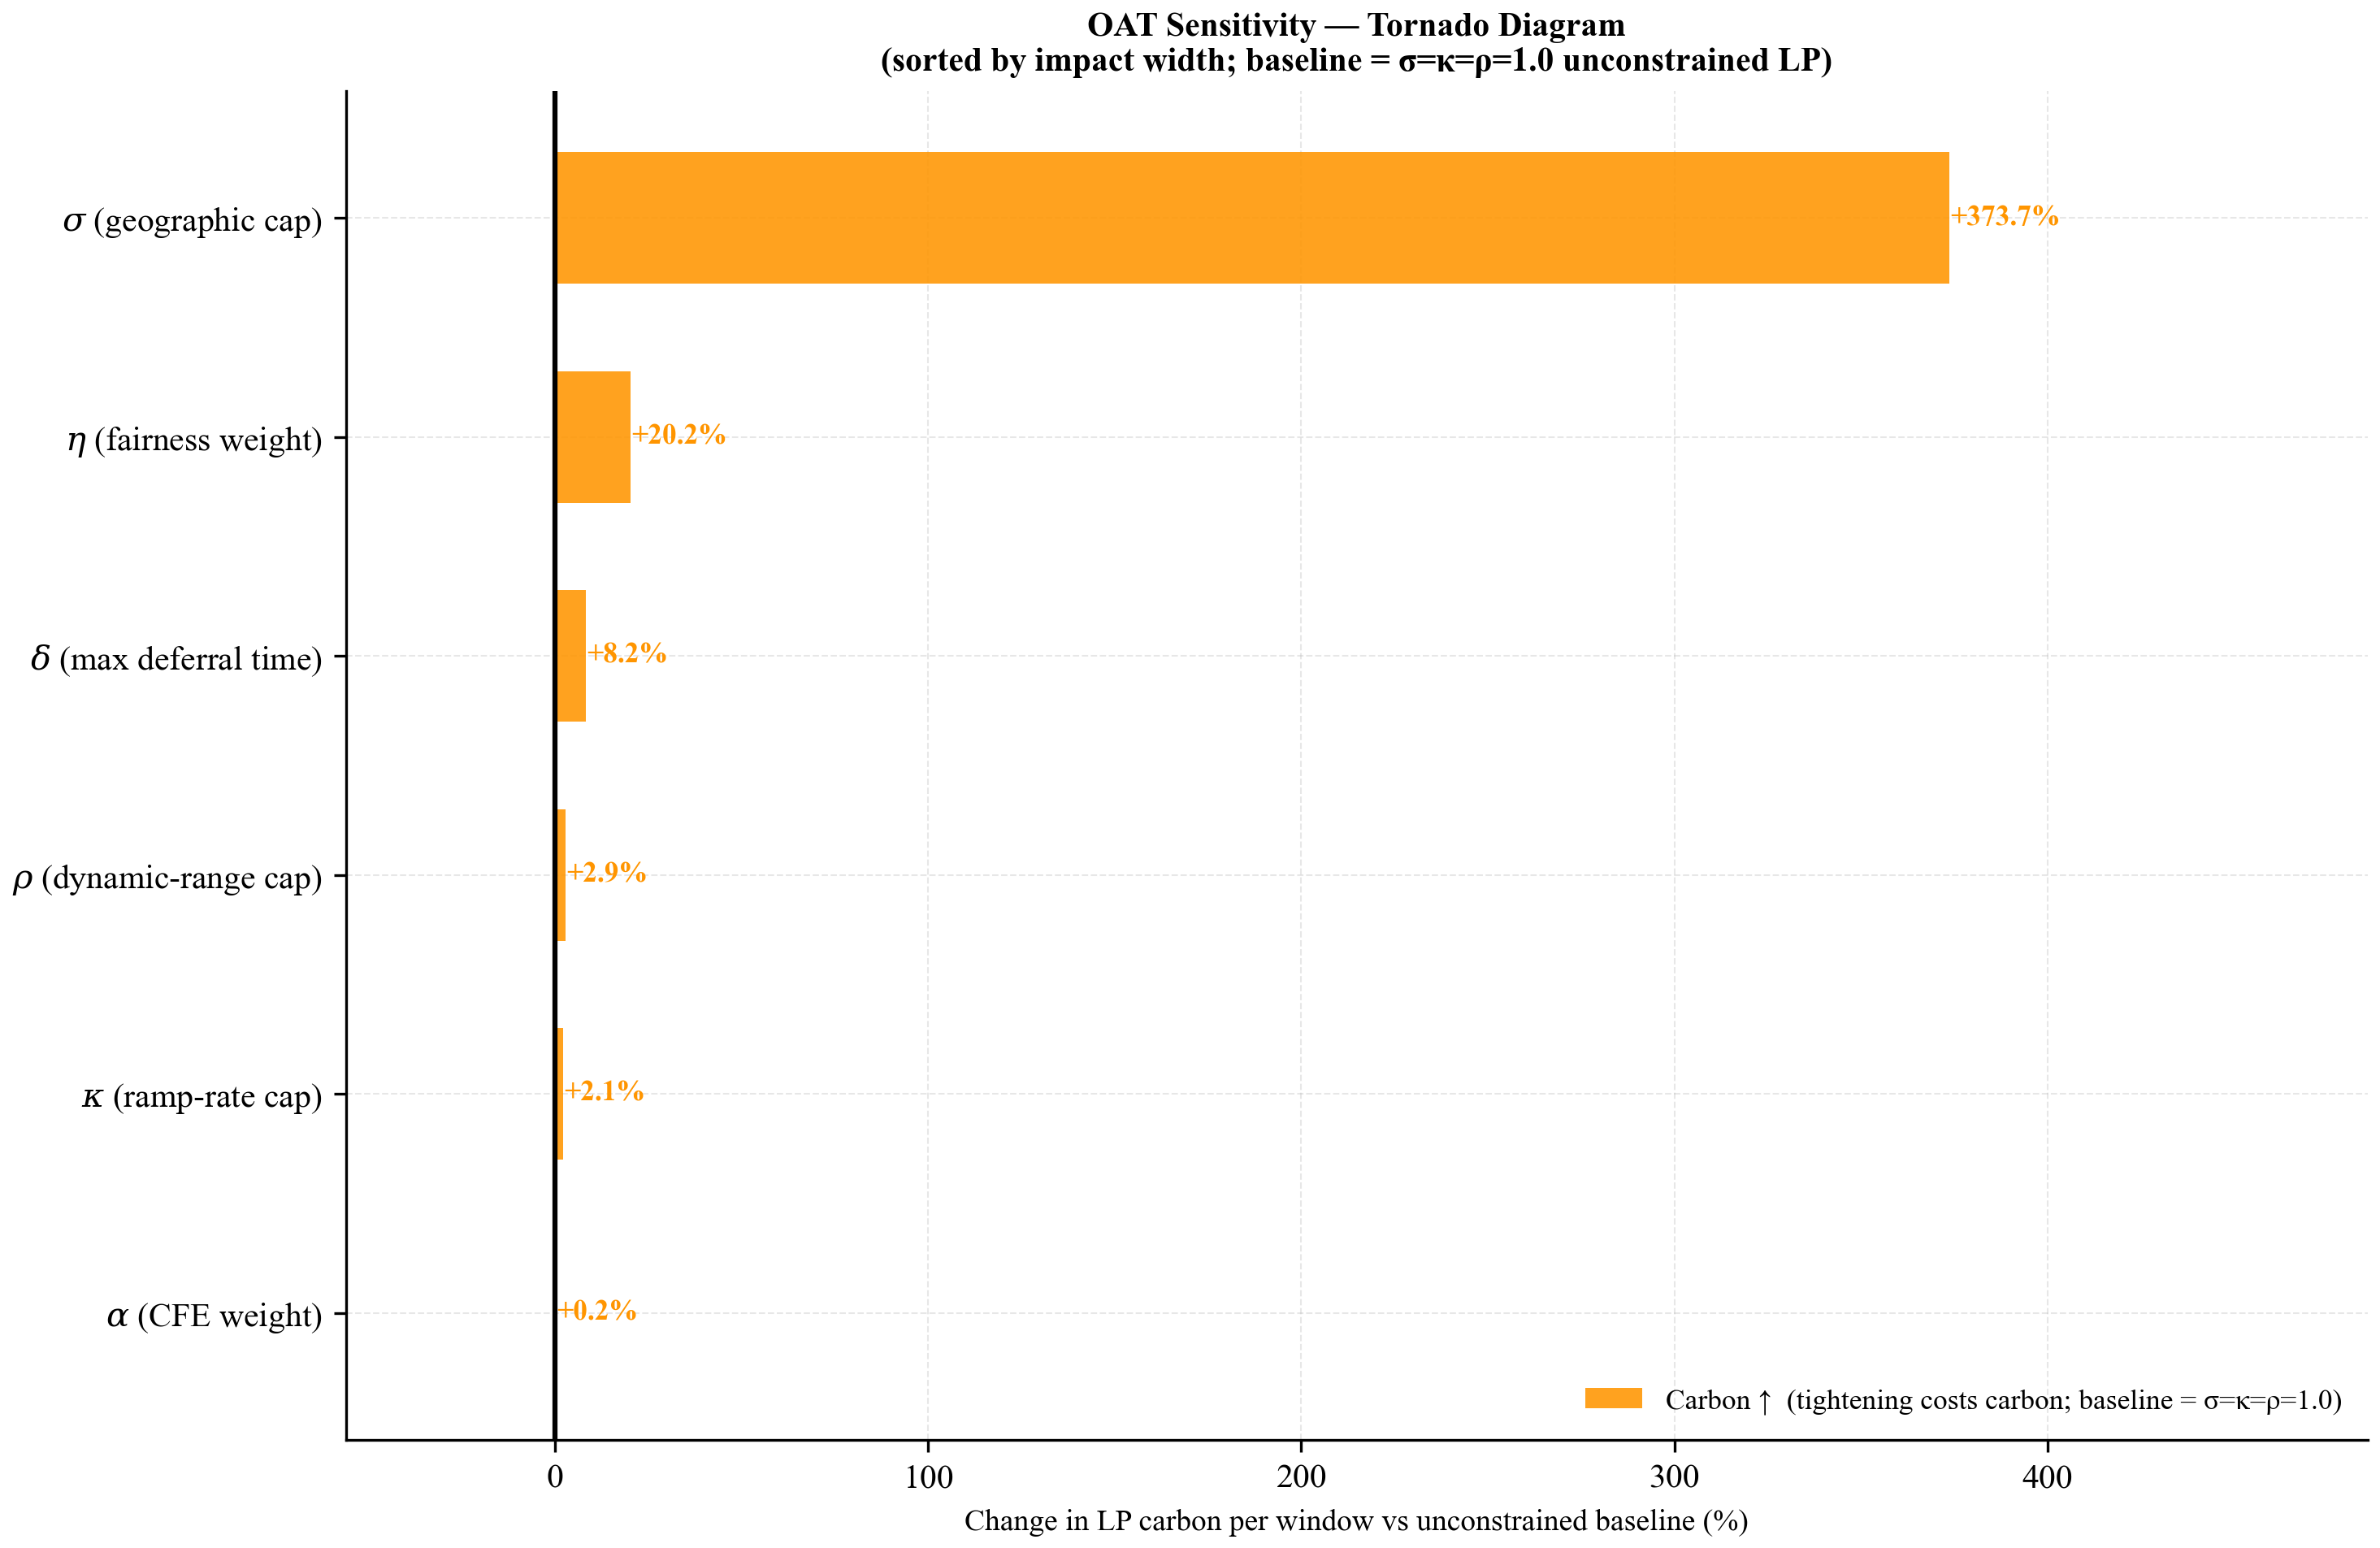
\includegraphics[width=\linewidth]{sensitivity_tornado}
\fcap{One-at-a-time sensitivity. Tightening the geographic cap $\sigma$ raises carbon by \textbf{+374\%}, against \textbf{+20\%} for equity $\eta$, \textbf{+8\%} for the deferral window $\delta$, and \textbf{$<$3\%} for $\rho,\kappa,\alpha$: how much load may move \emph{across regions} sets the ceiling on savings, not how it is shaped in time.}
\end{block}
\vfill
\begin{block}{\sn{13} Comparison with Practical Schedulers}
\centering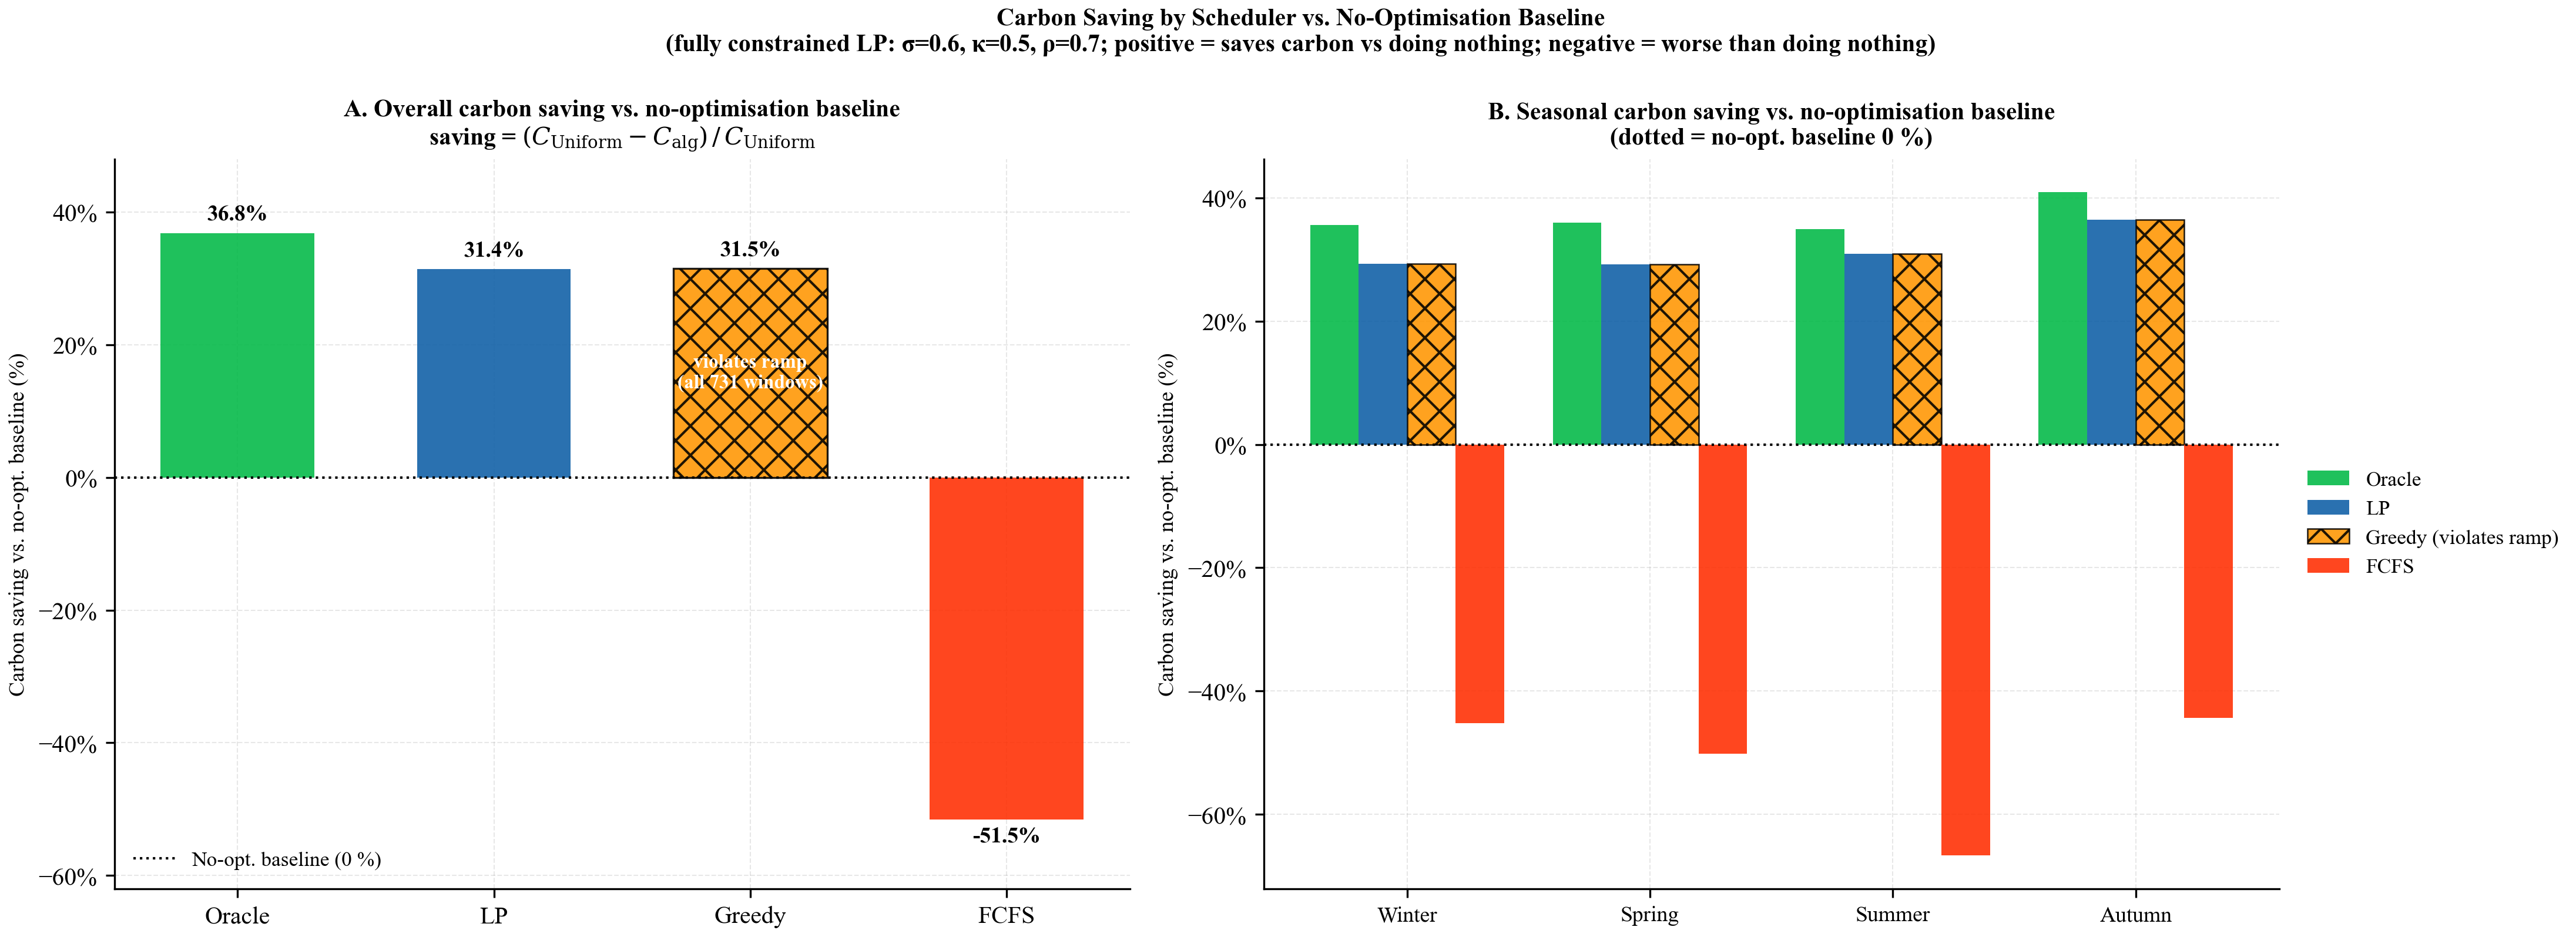
\includegraphics[width=\linewidth]{heuristic_comparison}\\[0.3ex]
{\renewcommand{\arraystretch}{1.3}
\begin{tabularx}{\linewidth}{@{}>{\raggedright\arraybackslash}X ccc@{}}
\rowcolor{pdark}\textcolor{white}{\textbf{Method}} & \textcolor{white}{\textbf{Save}} & \textcolor{white}{\textbf{Feasible}} & \textcolor{white}{\textbf{Foresight}}\\
Oracle & 36.8\% & \yes & week\\
\rowcolor{phl}\textbf{LP (this work)} & \textbf{31.4\%} & \yes & 24\,h\\
Greedy & 31.5\% & \no\,(ramp) & 24\,h\\
FCFS & $-51.5\%$ & \no & none\\
\bottomrule
\end{tabularx}}
\fcap{The LP is the only method that attains near-ceiling savings \emph{and} provably respects every constraint; greedy matches its carbon only by violating the ramp limit (all 731 windows).}
\end{block}
\vfill
\begin{block}{\sn{14} Where the Savings Come From}
\centering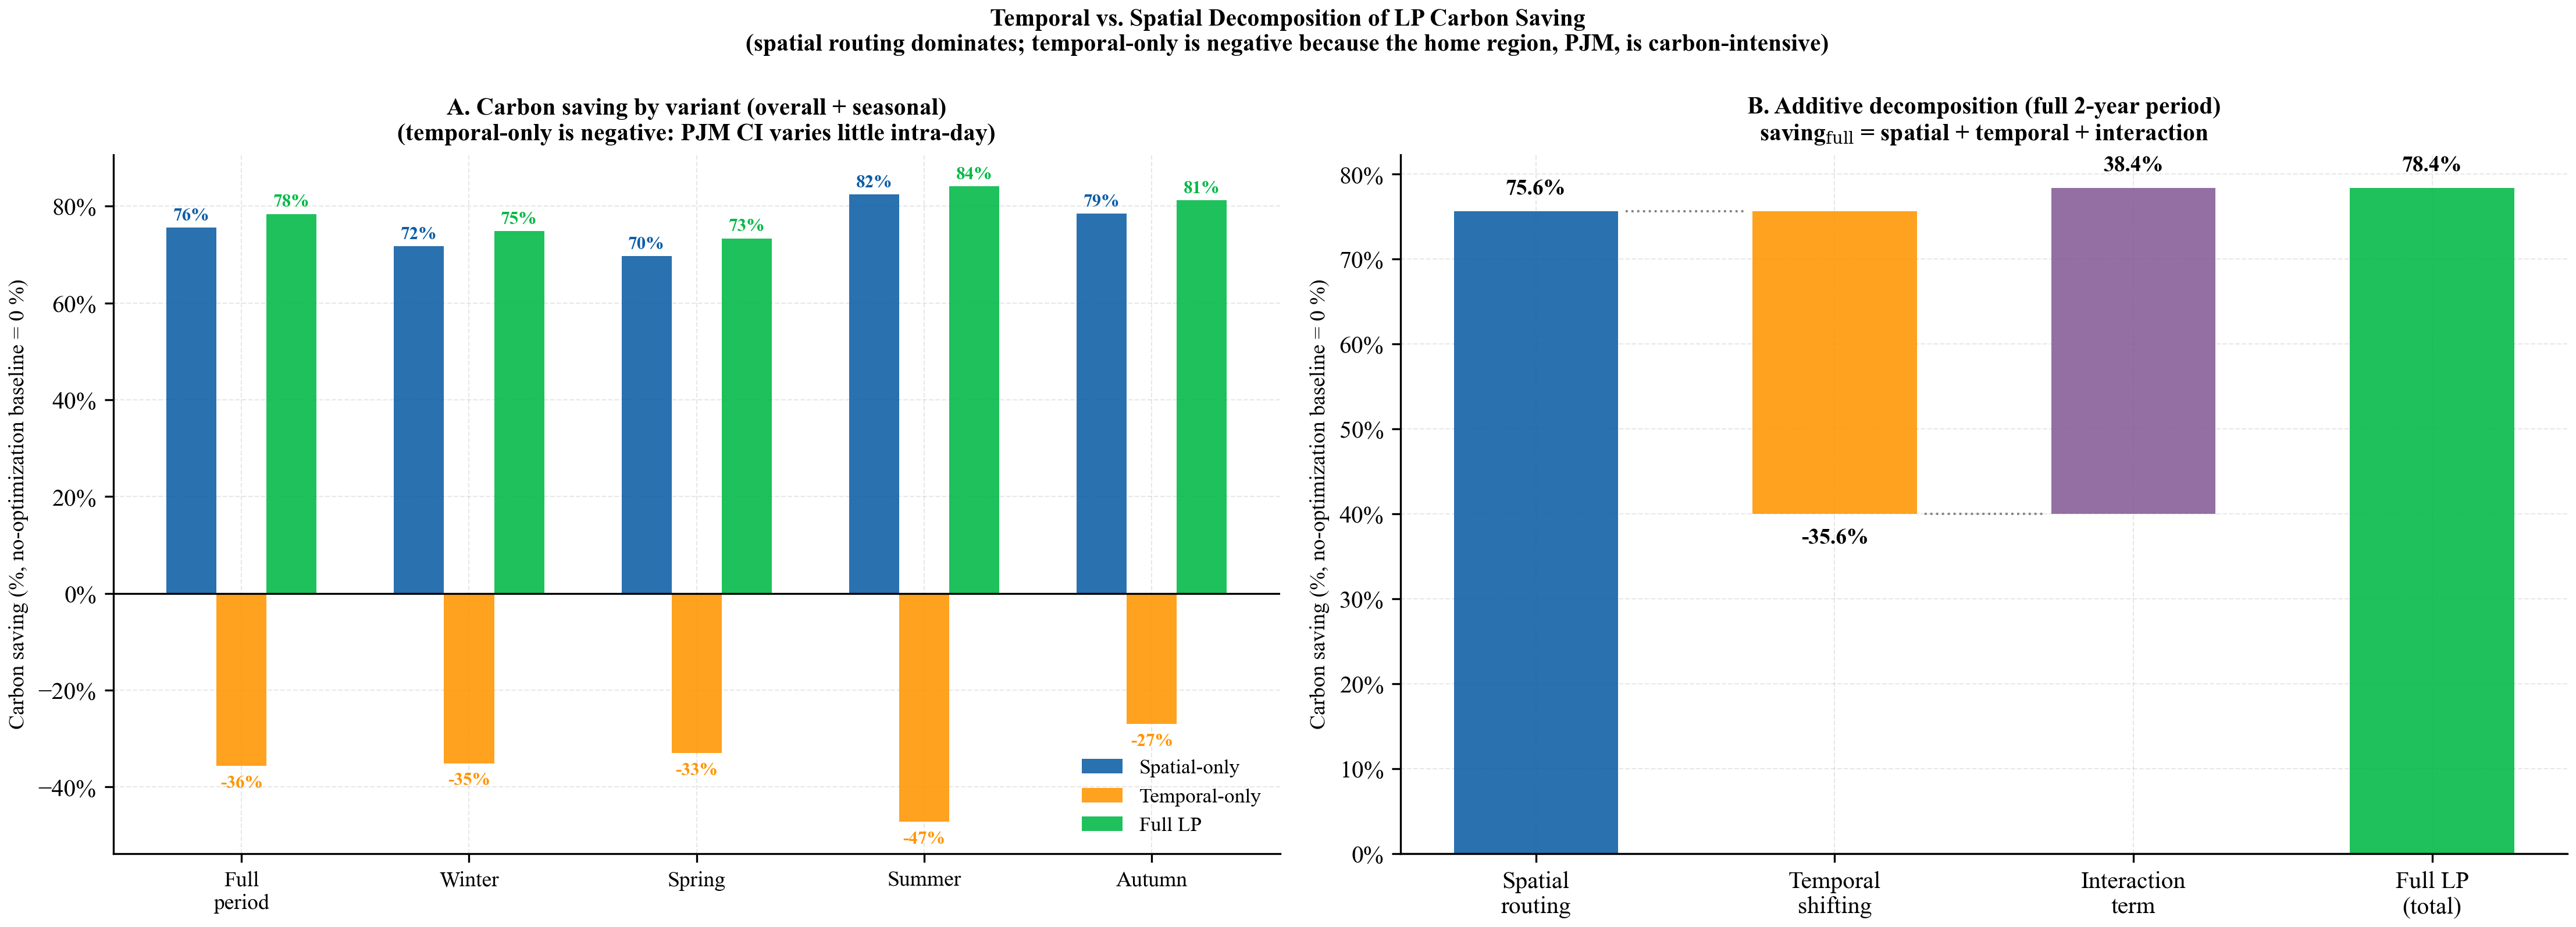
\includegraphics[width=\linewidth]{decomposition}\\[0.2ex]
\centering
\textbf{\textcolor{pgreen}{+75.6\%} routing}\ \ \textbf{\textcolor{pred}{$-$35.6\%} timing}\ \ \textbf{\textcolor{pmid}{+38.4\%} interaction}
\fcap{Routing accounts for almost all of the saving; time-shifting \emph{alone} can increase carbon. The two are strongly complementary.}
\end{block}
\vfill
\begin{block}{\sn{15} Seasonal Robustness}
\centering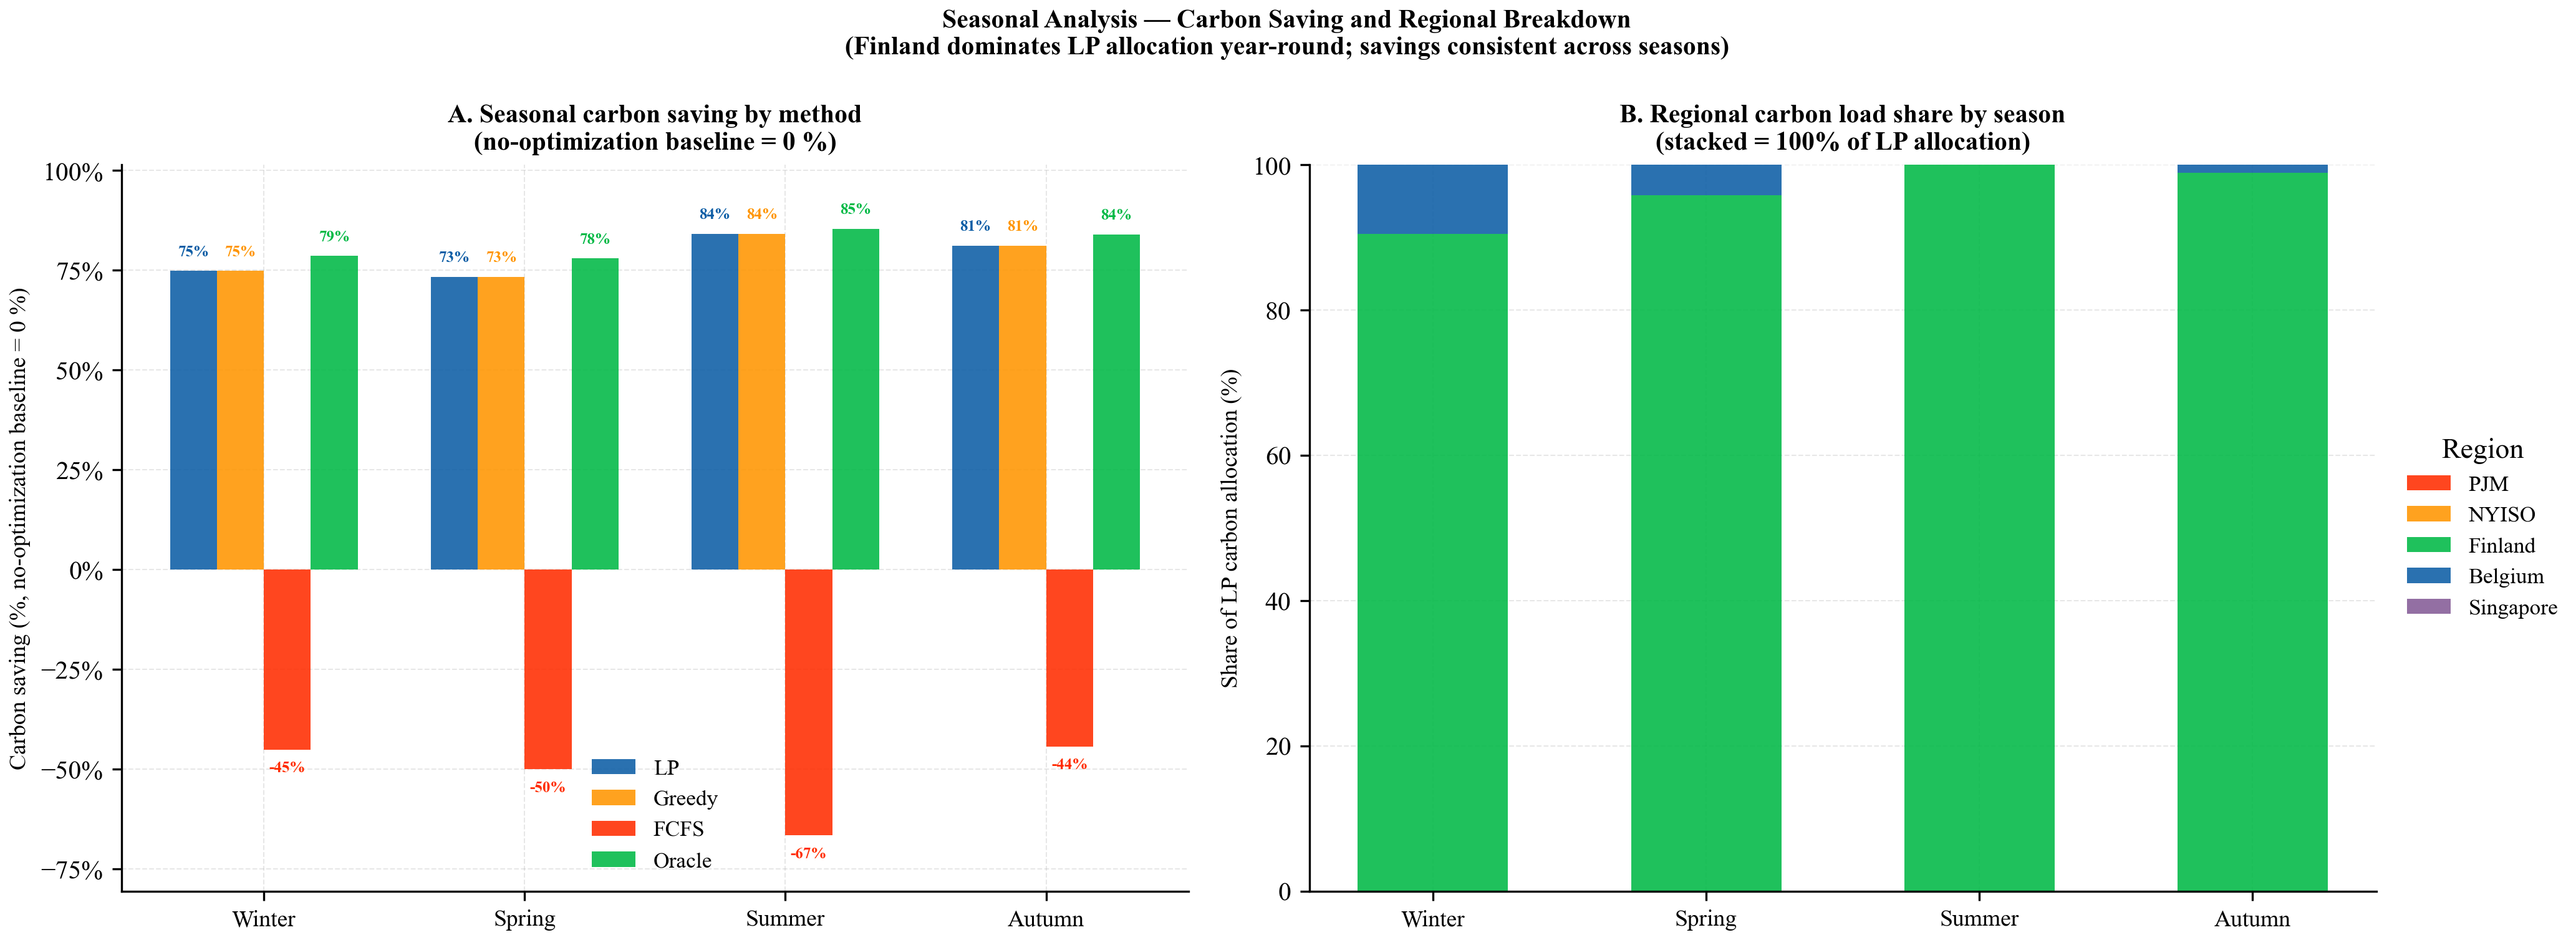
\includegraphics[width=\linewidth]{seasonal_breakdown}
\fcap{Savings are stable across seasons (\textbf{73--84\%}); Finland dominates the allocation year-round. The result is not an artefact of one season.}
\end{block}

\end{minipage}
\end{column}
\end{columns}

% ── Slim footer (future work) ───────────────────────────────────────────────
\vspace{0.15cm}
\begin{beamercolorbox}[wd=\paperwidth,sep=0.3cm,rounded=true]{block title}
\centering\small
\textbf{Future work:}\ marginal emissions \ \textbullet\ \ forecast uncertainty \ \textbullet\ \ water co-optimization \qquad\textbf{Data:}\ ElectricityMaps 2024--2025 \ \textbullet\ \ \textbf{Solver:}\ HiGHS LP
\end{beamercolorbox}

\end{frame}
\end{document}
